\documentclass[a4paper,12pt]{report}

\usepackage{graphicx}
\usepackage[spanish, es-tabla]{babel} % Para separar correctamente las palabras, es-tabla: para que nombre a la tabla como tal y no cuadro.

\usepackage[utf8]{inputenc} % Este paquete permite poner acentos y eñes usando codificación utf-8
\usepackage{setspace}
\onehalfspace %para espacio y medio

\usepackage{fancyhdr} %encabezado y pie de pag
\usepackage{framed} %recuadros de texto
\usepackage{multicol} %colocar texto en columnas

\usepackage{amsmath}%formulas y funciones mat

\newcommand{\at}{\makeatletter @\makeatother}%comando define la arroba porque no forma parte de latex

%=====formato para escribir pseudo-algortimo.============
%algorithm2e: para que ande 'sudo apt-get install texlive-science'
%aqui se encuentra instalado:
%/usr/share/texmf-texlive/tex/latex/algorithm2e/algorithm2e.sty
\usepackage[spanish,ruled,vlined,onelanguage]{algorithm2e} 
%ruled, vlined para formato de lineas.  
%spanish setea idioma español
%onelanguage español las palabras reservadas
%===================================================

%Encabezado
\lhead[]{\leftmark}
\chead[]{}
\rhead[]{\thepage}
\renewcommand{\headrulewidth}{0pt}

%Pie de pag
\lfoot[]{}
\cfoot[]{}
\rfoot[]{}
\renewcommand{\footrulewidth}{0pt}

%Setea configuracion enc y pie de pag
\pagestyle{fancy}


\begin{document}

\begin{titlepage}
    \centering
    \vfill
    {\bfseries\huge
	Análisis de Identificadores para Abstraer conceptos del 		Dominio del Problema
     \vskip1.3cm       
   }  
   
{\bfseries\Large

Trabajo Final de Licenciatura en Ciencias de la Computación
\vskip1cm
}

 {\bfseries\large
	Autor
	\vskip0.1cm   
   }
   {\bfseries\Large
Javier Azcurra Marilungo
   \vskip1cm
   }
%=========   
   {\bfseries\large
	Director
	\vskip0.1cm   
   }
   {\bfseries\Large
Dr. Mario Marcelo Berón
   \vskip1cm
   }
%=========   
   {\bfseries\large
	Co-Director
	\vskip0.1cm   
   }
   {\bfseries\Large
Dr. Germán Antonio Montejano
   \vskip1cm
   }

{\bfseries\large
Departamento de Informática
\vskip0.5cm
Facultad de Ciencias Físico Matemáticas y Naturales
\vskip0.5cm
Universidad Nacional de San Luis
%\vskip0.5cm
%
\includegraphics[width=1cm]{unsl_logo.jpg} 
}     
  
\end{titlepage}

\renewcommand{\abstractname}{\Large Resumen}

\begin{abstract}

Las demandas actuales en el desarrollo de software implican una evolución y mantenimiento constante con el menor costo de tiempo y de recursos. La ingeniería del software (IS) se encarga de llevar adelante esta tarea. Dentro de la IS existe el área de Comprensión de Programas (CP). Esta área se dedica a agilizar la comprensión de los sistemas de software, en base al desarrollo de  Métodos, Técnicas, Estrategias y Herramientas. 

%Una área de la CP es la extracción de información estática, la misma permite recolectar componentes relevantes del código sin necesidad de ejecutar el programa. Un componente conocido que abundan en los códigos son los identificadores (ids). 
La extracción de la información es un área de investigación muy usada por la CP. Esta área tiene como uno de sus principales objetivos la recolección de diferentes elementos del programa, los cuales pueden ser utilizados para diferentes propósitos en el contexto de CP. Los identificadores son uno de tales elementos.
Estudios indican \cite{BCPT99,LFBEX07,EZH08,EHPV09} que los ids esconden detrás de sus abreviaturas indicios de las funcionalidades de los sistemas. Por ende, cons\-truir herramientas automatizadas que extraigan y analicen ids es relevante para facilitar la comprensión de programas. La extracción de ids es lo más sencillo y una forma de lograrlo es con un parser construido a medida.
Sin embargo, el análisis del significado de los ids en el código fuente es más complicado por que el nombramiento de estos depende de cada programador. Una estrategia para analizar ids es expandir las abreviatura que lo componen.%CONSULTAR

La expansión de las abreviaturas del id a palabras completas es compleja, pero si se hace correctamente puede ayudar a comprender el sistema. Para lograr esta expansión, se emplean recursos propios del programa de estudio: comentarios, literales, documentación o bien, con fuentes externas al sistema basándose en diccionarios de palabras. 

%En este trabajo final de licenciatura, se describen técnicas conocidas que analizan ids en base a la expansión de sus abreviaturas. También se describe una herramienta desarrollada en JAVA llamada \mbox{\textit{Identifier Analyzer}} (IDA) que implementan algunas de estas estrategias. Luego, se explica los resultados obtenidos por la herramienta de acuerdo a distintos casos de estudio. Finalmente se arriba a conclusiones.

En este trabajo final de licenciatura, se describe \mbox{\textit{Identifier Analyzer}} (IDA) una herramienta útil para el análisis de identificadores de programas escritos en java. IDA implementa técnicas de expansión de las abreviaturas de los identificadores con el propósito de facilitar la comprensión de los sistemas de software. 

%Pensar en estrategias que faciliten las tediosas tareas que diariamente conllevan al crecimiento de los sistemas nos da incapie a iniciarnos en la investigación de herramientas automatizadas que posibiliten el reemplazo del esfuerzo manual que realizan los ingenieros de software a la hora de interpretar un programa.

\end{abstract}

%\renewcommand{\abstractname}{\Large Agradecimientos}
%
%\begin{abstract}
%\begin{multicols}{2}
%\begin{flushleft}
%\end{flushleft}
%\columnbreak
%\begin{flushright}
%\textit{“Hay en el mundo un lenguaje que todos comprenden: es el lenguaje del entusiasmo, de las cosas hechas con amor y con voluntad, en busca de aquello que se desea o en lo que se cree.”\linebreak Paulo Cohelo}
%\end{flushright}
%\end{multicols}
%\end{abstract}

\tableofcontents %Genera el indice

%CAPITULO1=============================================================

\chapter{Introducción: Problema y Solución}

Cuando se desarrollan los sistemas de software se busca que el producto final satisfaga las necesidades de los usuarios, que el buen funcionamiento perdure en el mayor tiempo posible y en caso de hacer una modificación para mejorarlo no implique grandes costos. Estos puntos conllevan a un software de alta calidad y la disciplina encargada de conseguirlo es la \mbox{\textit{Ingeniería de Software} (IS).}
% mbox obliga a mantener en la misma linea

La IS abarca, entre otras tantas, tres temáticas importantes que están orientadas al desarrollo de buenos sistemas: el \textit{mantenimiento del software}, la \textit{evolución del software} y la \textit{migración del software}. 

\section{Mantenimiento del Software}

La etapa de mantenimiento es importante en el desarrollo del software, por que está sujeto a cambios y a una permanente \mbox{evolución \cite{PFT02}.}

El mantenimiento del software según la IEEE standard \cite{STD610}, \textit{es la mo\-dificación del software que se realiza posterior a la entrega del producto al usuario con el fin de arreglar fallas, mejorar el rendimiento, o adaptar el sistema al ambiente que ha cambiado.}

De la definición anterior se desprenden 4 tipos de cambios que se pueden realizar en la etapa de mantenimiento. El \textit{mantenimiento correctivo} cambia el software para reparar las fallas detectadas por el usuario. El \textit{mantenimiento adaptativo} modifica el sistema para adaptarlo a cambios externos, como por ejemplo actualización del sistema operativo o el motor de base de datos. El \textit{ mantenimiento perfectivo} se encarga de agregar nuevas funcionalidades al software que son descubiertas por el usuario. Por último, el \textit{mantenimiento preventivo} realiza cambios al programa para facilitar futuras correcciones o adaptaciones que puedan surgir en el futuro \cite{RSPMGH02}.

%Es común también que por la constate actualización de los sistemas operativos, los motores de base de datos y demás sistemas externos que interactúan con el software desarrollado entren en conflicto, por eso en la fase de mantenimiento también se debe ir actualizando los distintos componentes del producto para una mejor compatibilidad\cite{RSPMGH02}. 

Por lo antedicho, entre otras diversas razones \cite{KBVR00} indican que el man\-tenimiento del software consume mucho esfuerzo y dinero. En algunos casos, los costos de mantenimiento pueden duplicar a los que se emplearon en el desarro\-llo del producto. Las causas que pueden aumentar estos costos son, el mal diseño de la arquitectura del programa, la mala codificación, la ausencia de documentación.

No es descabellado pensar estrategias de automatización que puedan ser aplicadas en fases del mantenimiento del software que ayuden a reducir estos costos, lo cual requiere una comprensión del objeto que se va a modificar antes de realizar algún cambio que sea de utilidad.
 
Algunos autores \cite{KBVR00,MAS05,RSPMGH02,PFT02} concluyen que el mantenimiento del software y la comprensión de los programas son conceptos que están fuertemente relacionados. Una frase conocida en la jerga de la IS es: \textit{“Mientras más fácil sea comprender un sistema, más fácil será de mantenerlo”}.


\section{Evolución del Software}

Los sistemas complejos evolucionan con el tiempo, los nuevos usuarios y requisitos durante el desarrollo del mismo causan que el producto final posiblemente no sea el que se planteó en un comienzo. 

La evolución del software básicamente se atribuye al crecimiento de los sistemas a través del tiempo, es decir, tomar una versión operativa y generar una nueva versión ampliada o mejorada en su eficiencia \cite{KBVR00}.

Generalmente, los ingenieros del software recurren a los modelos evolutivos. Estos modelos indican que cuando se desarrolla un producto de software es conveniente que se divida en distintas iteraciones. A medida que avanza el desarrollo, cada iteración retorna una version entregable cada vez más compleja \cite{RSPMGH02}. 

Estos modelos son muy recomendados sobre todo si se tienen fechas ajustadas donde se necesita una versión funcional lo más rápido posible. De esta manera, no se requiere esperar una versión completa al final del proceso de desarrollo.

Es imperioso y fundamental comprender correctamente la iteración actual del producto antes de comenzar con una nueva. Nuevos requerimientos del usuario pueden aparecer, como así también nuevas dificultades en el desarrollo del sistema. Es por esto que la comprensión del sistema durante su evolución es crucial.

%Los integrantes en el proceso de desarrollo pueden ir variando durante las distintas iteraciones y teniendo en cuenta que se va acomplejando cada vez más, la comprensión del sistema durante la evolución representa un verdadero desafío.


\section{Migración del Software}

Las tareas de mantenimiento de software no solo se realizan para mejorar cuestiones internas del sistema, como es el caso de arreglos de errores de programación o requisitos nuevos del usuario. También se necesitan para adaptar el software al contexto cambiante. Es aquí donde la \textit{migración del software} entra en escena.
 
De acuerdo con la IEEE standard \cite{STD1219}, \textit{la migración del software es convertir o adaptar un viejo sistema (sistema heredado) a un nuevo contexto tecnológico sin cambiar la funcionalidad del mismo}.

Las migraciones de sistemas más comunes que se llevan a cabo son causadas por cambios en el hardware obsoleto, nuevos sistemas operativos, cambios en la arquitectura y nuevas base de datos. Sin duda, la que más se ha acentuado en los últimos años son la aparición de nuevas tecnologías web y las mobile (basadas en dispositivos móviles) \cite{MMFAF07}.
 
La migración de grandes sistemas es fundamental, sin embargo está demostrado que es costosa y compleja \cite{MMFAF07}. Para llevarla a cabo reduciendo estos costos se recomienda hacer previamente una buena comprensión del sistema antiguo. 

Una técnica de comprensión de sistemas ideada recientemente para la migración de software, consiste en un mode\-lado de datos \cite{WHAFVR11}. Esta modelado se encarga de abstraer el código antiguo a niveles más altos, al hacerlo reduce los esfuerzos de comprensión. De esta forma, el grupo encargado de la migración solo debe preocuparse por convertir el antiguo código a la nueva tecnología.

Nuevamente la comprensión de programas se hace presente en temáticas relacionadas al desarrollo de proyectos de software.

\section{Comprensión de Programas}

Como se explicó en las secciones anteriores, es crucial lograr comprender el sistema para llevar adelante las tareas de mantenimiento, evolución y migración del software.	
Por esta razón, existe un área de la IS que se dedica al desarrollo de técnicas de inspección y comprensión de software. Esta área se conoce con el nombre de \mbox{\textit{Comprensión de Programas} (CP).}

La CP se define como: \textit{Una disciplina de la IS encargada de ayudar al desarrollador a lograr un entendimiento acabado del software. De forma tal que se pueda analizar disminuyendo en lo posible el tiempo y los costos} \cite{MPMR07}.  

La CP asiste al equipo de desarrollo de software proveyendo métodos, técnicas y herramientas que faciliten el entendimiento del sistema de estudio.

Las investigaciones realizadas en el área de la CP determinaron que el foco de estudio se centra en relacionar el \textit{Dominio del Problema} con el \textit{Dominio del Programa} \cite{BRM10,MPMR07,MBPHRU10,DWE04}. El primero hace referencia a los elementos que forman parte de la salida del sistema, mientras que el segundo indican las componentes del programa empleados para generar dicha salida.
Esta relación es compleja de realizar y representa el principal desafío de la CP. 

Una aproximación para relacionar ambos dominios consiste en elaborar la siguiente reconstrucción:

I) Armar una representación del \textit{Dominio del Problema}. II) Construir una representación para el \textit{Dominio del Programa}. III) Unir ambas representaciones con una \textit{Estrategia de Vinculación}.

Para llevar a cabo los 3 pasos mencionados, se necesitan estudiar temáticas asociadas a la CP. Las más importantes son:

\begin{itemize}
\itemsep0em%reduce espacio
\item Los \textit{Modelos Cognitivos} son relevantes para la CP porque destacan como el programador utiliza procesos mentales para comprender el software.

\item La \textit{Visualización del Software} analiza las distintas partes del sistema y genera representaciones visuales que agilizan la CP.

\item La \textit{Interconexión de Dominios} trata de como interrelacionar los elementos de un dominio con otro. Es útil para la CP en la reconstrucción de la relación entre dominio del problema y el dominio del programa.

\item La \textit{Extracción de Información} en los sistemas de software permite revelar información oculta en los programas que es valiosa para la CP. Es necesaria para las estrategias de cognición, visualización, interconexión de dominios, etc.

\item Al extraer gran cantidad de información se necesita la \textit{Administración de Información}. La misma brinda técnicas de almacenamiento y acceso a la información extraída.

\end{itemize}

Todos estos temas se explican con mayor precisión en el próximo capítulo. En la siguiente sección se amplia la \textit{extracción de la información} ya que es la antesala al \textit{análisis de identificadores}, eje central de este trabajo final.


%Una forma de alcanzar este objetivo consiste en relacionar el \textit{Dominio del Problema} con el \textit{Dominio del Programa}\cite{BRM10,MPMR07,MBPHRU10}. El primero hace referencia a los elementos que forman parte de la salida del sistema, mientras que el segundo indican las componentes del programa empleados para generar la salida del sistema.

%La construcción de esta relación es compleja y representa el principal desafío en el contexto de la CP. Una aproximación para alcanzar esta relación consiste en armar una representación del \textit{Dominio del Problema}, luego una representación para el \textit{Dominio del Programa} y finalmente unir ambas representaciones con una \textit{Estrategia de Vinculación}.

%La comprension de programas
%La visualizacion de software
%Extraccion de Información

%Problema y solucion


%De todos los problemas a los que se enfrentan los desarrolladores de software el primordial es el de mantener los sistemas en buen funcionamiento \cite{VMAVA95}. 
%Esta tarea es imposible de llevar a cabo de forma manual debido a que consume muchos costos y esfuerzo humano.
%==============================================================================

%Para construir   temáticas de Extracción de Información y la Visualización de Software\cite{MPMR07,STOREY99,BROOK82}.

\section{Extracción de Información}

En la CP, la \textit{Extracción de la Información} se define como \textit{el uso/desarrollo de técnicas que permitan extraer información desde el sistema de estudio}. 
Esta información puede ser: Estática o Dinámica, dependiendo de las necesidades del 
ingeniero de software o del equipo de trabajo.

La extracción de información estática recupera los distintos elementos en el código fuente de un programa \cite{AHUL06}. 

%Normalmente se utilizan técnicas de compilación tradicionales, que se encargan de recuperar información de cada componente del sistema. Todas las actividades que forman parte de esta tarea se realizan desde el código fuente sin ejecutar el sistema. 

%Generalmente, para este tipo de trabajos se construye un analizador sintáctico. Este analizador posee acciones semánticas que se encargan de extraer la información requerida.

Por otro lado, la extracción dinámica de información implica obtener los elementos que se utilizaron en la ejecución del sistema \cite{THBE99}. Generalmente no todas las partes del código son ejecutadas, por lo tanto no todos los elementos se pueden recuperar en una sola ejecución.

%Para extraer información dinámicamente se utiliza las técnicas de instrumentación de código. Estas técnicas, consisten en insertar sentencias dentro del código fuente con el fin de recuperar las partes del programa que se utilizaron para producir la salida.
 
La principal diferencia que radica entre ambas técnicas,  es que las estáticas se basan en la información presente en el código, mientras que las dinámicas es obligatorio ejecutar el sistema.
A veces, se recomienda complementar el uso de ambas estrategias para obtener mejores resultados \cite{TERD01}.

%Una vez extraída la información necesaria se pueden elaborar estrategias de visualización de software para explayar la información obtenida.

%\section{Visualización de Software}

%La \textit{Visualización del Software} es una característica importante en la comprensión de programas por que ayuda a representar visualmente la información de los sistemas de software\cite{BRM10}. Con esto se simplifica la comprensión del software y de esta manera se facilita el mantenimiento, la evolución y la migración de los sistemas.

%Con la visualización de software se puede implementar sistemas de visualización. Estos sistemas brindan información a través de las vistas. Dichas vistas, cuando están bien elaboradas, permiten analizar y percibir la información extraída desde un programa con mayor facilidad.

%Para aclarar aun más este punto, si se implementan buenos sistemas de visualización, se pueden lograr una correcta representación del dominio del problema, del dominio del programa y de la estrategia que vincula ambas representaciones que se explicó con anterioridad.

% Un concepto clave para vincular la representación de ambos dominios es la Interconexión de Dominios.


%\section{Interconexión de Dominios}

%La Interconexión de Dominios tiene como principal objeto de estudio la transformación y vinculación de un dominio específico en otro dominio\cite{MPMR07}. 
%Este último dominio puede estar en un alto o bajo nivel de abstracción. 
%El punto importante es que cada componente de un dominio se vea reflejado en una o más componentes del otro y viceversa. 
%A modo de ejemplo, se puede mencionar la transformación de un código fuente (Dominio del Programa) en un Grafo de Llamadas a Funciones (Dominio de Grafos). En este contexto existe una amplia gama de transformaciones siendo la más escasa y difícil de conseguir aquella que relaciona el Dominio del Problema con el Dominio del Programa.
 
%Para construir herramientas de comprensión, se deben tener en cuenta cuatro pilares importantes: \textit{Modelos Cognitivos}
%\textit{Extracción de la Información},
%\textit{Interconexión de Dominios} y la
%\textit{Visualización de Software} \cite{STOREY99,BROOK82}.
%
%
%Los \textit{Modelos Cognitivos} se refiere a las estrategias de estudio y las estructuras de información usadas por los programadores para comprender los programas. Están formados por distintos componentes: Conocimiento, un modelo mental y un proceso de asimilación.
%Existen dos tipos de conocimientos uno es el interno que constituye los conocimientos que el programador tiene incorporado y el otro es el Externo en donde el sistema a estudiar provee al desarrollador nuevos conceptos.
%El modelo mental es la representación mental que el programador tiene sobre el sistema. Algunos modelos conocidos por los arquitectos del software como el \textit{Unified Modeling Language} UML, \textit{Entity Relationship} ER entre otros pueden verse como representaciones de modelos mentales.
%Por último, el proceso de asimilación engloba la estrategia que utiliza el programador para entender los programas. Ellas son Bottom-up, Top-Down e Hibrida.
%Varios autores concluyen que estos conceptos conforman la base para encontrar la relación entre el dominio del problema y el dominio del programa\cite{TIE89,MPOB03}.
%
%
%La \textit{Visualización del Software} es una característica importante en la comprensión de programas, básicamente provee una o varias representaciones visuales (o vistas) de algún sistema particular \cite{BRM10}.
%Dichas vistas, cuando están bien elaboradas, permiten analizar y percibir la información extraída desde un programa con mayor facilidad.
%Para lograr lo antedicho se utilizan librerías gráficas conocidas, algunas de ellas son Jung, Prefuse, Graphviz y Cairo.
%Cabe destacar que el diseñador de la visualización debe hacer un análisis profundo para seleccionar la librería mas adecuada.
%La visualización de software orientada a la comprensión de programa tiene como principal desafío generar vistas que ayuden a relacionar el Dominio del Problema con el Dominio del Programa.
%
%La \textit{Interconexión de Dominios} \cite{BRM10} tiene como principal objeto de estudio la transformación y vinculación de un dominio específico en otro dominio. 
%%Este último dominio puede estar en un alto o bajo nivel de abstracción. 
%El punto importante es que cada componente de un dominio se vea reflejado en una o más componentes del otro y viceversa. 
%A modo de ejemplo, se puede mencionar la transformación de un código fuente Dominio del Programa) en un Grafo de Llamadas a Funciones (Dominio de Grafos). En este contexto existe una amplia gama de transformaciones siendo la más escasa y difícil de conseguir aquella que relaciona el Dominio del Problema con el Dominio del Programa.
%
%Por \textit{Extracción de la Información} se entiende el uso/desarrollo de técnicas que permitan extraer información desde el sistema de estudio. 
%Esta información puede ser: Estática o Dinámica, dependiendo de las necesidades del 
%ingeniero de software o del equipo de trabajo.
%Para la extracción de la información estática se utilizan técnicas de compilación tradicionales, que se encargan de recuperar información de cada componente del sistema. Todas las actividades que forman parte de esta tarea se realizan desde el código fuente sin ejecutar el sistema. Generalmente, en este tipo de trabajos se construye un analizador sintáctico con las acciones semánticas necesarias para extraer la información requerida.
%Por otro lado la extracción dinámica de información del sistema se obtiene  
%aplicando técnicas de instrumentación de código, estas técnicas consisten en insertar sentencias dentro del código fuente del sistema con el fin de recuperar las partes del programa que se utilizaron para 
%producir la salida. 
%La principal diferencia que radica entre ambas técnicas es que las dinámicas requieren que el sistema se ejecute, mientras que las estáticas esto no es necesario.
%
% 
%
%\textbf{Concluimos que tanto la representación del dominio del problema como la representación del dominio del programa se construye en base a la información, estática y dinámica, que se extrae de los mismos. 
%La estrategia de vinculación usa esa información para construir un mapeo entre los elementos de ambos dominios.}


%En el correspondiente trabajo se describe una línea de investigación que tiene como principal foco de estudio el análisis y la implementación de técnicas de extracción de la información estática en los sistemas de software que permitan aproximar a la construcción de la relación entre el Dominio del Problema y el Dominio del Programa.



%Finalmente, es importante mencionar que la información dinámica es tan importante como la información estática, sin embargo su extracción requiere del estudio de otro tipo de aproximaciones que conforman en sí otra línea de investigación.

%Los párrafos precedentes permiten percibir la importancia de las técnicas de extracción de la información. 
%Sin ellas no sería posible la construcción de visualizaciones y técnicas de interconexión de dominios\cite{BRM10,MPMR07}.

En este trabajo final se hace énfasis en la extracción de información estática. Es importante aclarar que la información dinámica es tan importante como la información estática, sin embargo su extracción requiere del estudio de otro tipo de aproximaciones y escapan al alcance de este trabajo.

Como se mencionó previamente, en los códigos de software abundan componentes que conforman la información estática. Alguno de ellos son, nombres de variables, tipos de las variables, los métodos de un programa, las variables locales a un método, constantes. Todos estos componentes se representan mediante los identificadores (ids). Los ids abarcan gran parte de los elementos de un código por lo tanto su análisis no debe pasarse por alto. 

%Esto se debe a que dicha información se encuentra expresada en lenguaje natural y por lo tanto su interpretación escapa del análisis estático y requiere de la aplicación de \textit{Técnicas de Procesamiento de Lenguaje Natural} \cite{DCPHJP09,TERD01}.

%El análisis de los ids representa el foco de estudio de este trabajo.

\section{Análisis de Identificadores}

Estudios realizados \cite{DFPM05,DMDJ13,HDD06,FBL06} indican que gran parte de los códigos están conformados por identificadores (ids), por ende abundante información estática está representada por ellos (ver capítulo 3).

Generalmente, los ids están compuestos por más de una palabra en forma de abreviaturas. Varios autores coinciden \cite{BCPT99,LFBEX07,EZH08,EHPV09} que detrás de estas abreviaturas, se encuentra oculta información que es propia del dominio del problema.

Una vía posible para exponer la información oculta consiste en traducir las abreviaturas antes mencionadas, en sus correspondientes palabras expresadas en lenguaje natural.

Para conseguir la traducción antedicha, I) primero se extraen los identificadores del código, II) luego se les aplica técnicas de división en donde se descompone al identificador en las distintas palabras abreviadas que lo componen. Por ejemplo: \textsf{inp\_fl\_sys} $\rightarrow$ \textsf{inp fl sys}. Finalmente, III) se emplea estrategias de expansión a las abreviaturas para transformar las mismas en palabras completas. Siguiendo con el ejemplo anterior: \textsf{inp fl sys} $\rightarrow$ \textsf{input file system}.

%Sin embargo, a través del estudio del estado del arte, se pudo detectar que son pocas las estrategias de análisis estático que analizan la información informal que se encuentra disponible en el código fuente, por información informal se entiende aquella contenida en los comentarios de los módulos, comentarios de las funciones, literales strings y documentación del sistema.

%Este trabajo se centra en los \textit{identificadores} ids como fuente principal de información.


Normalmente, los nombres de los ids son elegidos en base a criterios del programador \cite{LFBEX07, EHPV09}. Lamentablemente, estos criterios son desconocidos para las técnicas de expansión de abreviaturas de ids.

%Otro problema a tener en cuenta es que las abreviaturas representan palabras en lenguaje natural, el cual es ambiguo y puede generar controversia en la conversión.

Para afrontar la dificultad que implica revelar los nombres abreviados de los ids, se recurre a fuentes de información informal que se encuentran disponible en el código fuente. Por información informal se entiende aquella contenida en los comentarios de los módulos, comentarios de las funciones, literales strings, documentación del sistema y todos lo demás recursos descriptivos del programa que estén escritos en lenguaje natural.

%Por lo tanto se necesita la ayuda de fuentes que contengan información informal presentes en el código que aporten en el proceso de la traducción de los ids. Los candidatos serios a lograr este cometido son comentarios y los literales string.
%Dicho de otra manera, son una fuente importante de información de los conceptos del Dominio del Problema.

Sin duda, los comentarios tienen como principal finalidad ayudar a comprender un segmento de código \cite{JDPH08}. Por esta razón, se puede ver a los comentarios como una herramienta natural para entender el significado de los ids en el código, como así también el funcionamiento del sistema.

Por otro lado para poder entender la semántica de los ids, se toman li\-terales o constantes strings.
Estos representan un valor constante formado por secuencias de caracteres. Ellos son generalmente utilizados en la muestra de carteles por pantalla, y comúnmente se almacenan en variables de \mbox{tipo string.}

Los literales string como los comentarios pueden brindar indicios del significado de las abreviaturas que se desean expandir.%, sin embargo se debe considerar que estos están escritos en lenguaje natural por lo tanto su co\-rrecta interpretación puede dificultarse por la ambigüedad.

En caso de que estas fuentes de información informal sean escasas dentro del mismo sistema, se puede acudir a alternativas externas como es el caso de los diccionarios predefinidos de palabras en lenguaje natural.

En la actualidad se puede clasificar a las estrategias que analizan id en 2 grandes grupos. Las que usan diccionarios predefinidos y las que no. Las primeras son las más arcaicas, mientras que las segundas son las más recientes.

Desafortunadamente, las estrategias de análisis de ids en su gran mayoría, no han sido implementadas en herramientas que integren las distintas características que implica la traducción de ids: dividir las abreviaturas que componen un id, expandirlas en base a lo observado en comentarios, utilizar diccionarios, etc.

\pagebreak
\section{Problema y la Solución}

Si bien existen técnicas/herramientas que extraen ids, dividen y expanden abreviaturas. No existen implementaciones que integren todas estas acciones en una única herramienta.

A su vez, tampoco hay herramientas que implementan distintas opciones de estrategias de división y de expansión de abreviaturas. De esta manera, se espera mejorar los resultados obtenidos por las aproximaciones actuales.

Para abordar las iniciativas planteadas y hacer algunos aportes a la solución de estos problemas planteados, se pretende:

\begin{itemize}
\itemsep0em%reduce espacio
\item Construir un analizador sintáctico en lenguaje Java que permite extraer los ids, comentarios y literales encontrados en el código fuente del sistema de estudio. La herramienta a seleccionar para realizar esta tarea es ANTLR\footnote[1]{ANother Tool for Language Recognition - http://www.antlr.org}.

\item Armar un diccionario de palabras en lenguaje natural que sirva como alternativa a las fuentes de información informal.

\item Investigar técnicas de división de ids y técnicas expansión de abreviaturas. Algunas de estas utilizan como principal recurso la información brindada en los comentarios y los literales extraídos del código. Como segunda posibilidad se recurre al diccionario.

\item Implementar empleando el lenguaje JAVA algunas de las técnicas del item anterior en una herramienta denominada \textit{Identifier Analyzer} (IDA). Esta herramienta también permite visualizar atributos del id (ambiente, tipo de identificador, número de línea, etc) mostrando la parte del código donde se encuentra ubicados.

%\item Graficar los resultados obtenidos....

\item Comparar el desempeño de cada técnica implementada en IDA y sacar las conclusiones pertinentes.

\end{itemize}

\pagebreak 
\section{Contribución}

El correspondiente trabajo final es un aporte al área de CP que basa su estudio sobre como capturar conceptos del dominio del problema a través del análisis de los ids en programas escritos en JAVA. 
%CONSULTAR

Este análisis consiste en técnicas de traducción de ids a palabras completas considerando distintas fuentes de información informal, como es el caso de los comentarios, los literales o diccionarios predefinidos de palabras. Luego algunas técnicas se implementan en una sola herramienta para comparar el desempeño con distintos casos de estudio.

%Finalmente se extraen conclusiones en base a los resultados obtenidos y se determinan posibles trabajos futuros sobre la investigación realizada.

%se buscan estrategias basadas en el análisis de los ids que faciliten la comprensión de programas haciendo así un pequeño aporte en la solución a la problemática de vincular ambos dominios mencionados. Esta información es muy importante porque facilita  la reconstrucción de la relación del Dominio del Problema con el Dominio del Programa\cite{DWE04}.

%\begin{itemize}
%
%\item Se investigaron herramientas de construcción de Analizadores Léxicos y Analizadores Sintácticos que emplean la teoría asociada a las gramáticas de atributos. 
%De la investigación mencionada previamente,  
%se determinó que la herramienta \textit{ANTLR}\footnote[1]{http://www.antlr.org/} es la más adecuada para extraer eficazmente los ids y toda la información relevante asociada a ellos que facilite su análisis.
%
%\item Se construyó un analizador sintáctico del lenguaje Java que permite extraer los ids, comentarios y literales encontrados en el código fuente del sistema de estudio.
%
%\item  Se estudiaron y se implementaron las técnicas de división de ids Greedy, Random \cite{HDD06,FBL06} que se encargan de separar a los ids en partes, donde cada parte representa una palabra abreviada.
%
%\item Se investigaron y se implementaron técnicas de expansión de ids en donde las abreviaturas previamente divididas se expanden en palabras completas.  
%Dichas técnicas llevan a disponer de listas de palabras formadas de los comentarios y literales capturados, (como así también una lista de palabras del diccionario en español).
%
%\item Se implementó una herramienta \textit{Identifier Analyzer} (IDA) que permite visualizar los atributos (ambiente, tipo de identificador, número de línea,etc) de cada objeto mostrando la parte del código donde se encuentra ubicados. Se incorporó en la implementación ademas las técnicas mencionadas en los ítems anteriores usando \textit{ANTLR} como herramienta soporte para la extracción de información.
%
%\end{itemize}


%======================================================================

\section{Organización del Trabajo Final}
%En este trabajo final se presenta una línea de investigación que se centra en el estudio, creación e implementación de técnicas de extracción de la información estática desde los sistemas de software. 
%Esta información puede ser estrictamente relacionada con el código del programa, o bien con la información informal provista por los programadores a través de comentarios, literales y documentación. 

El trabajo está organizado de la siguiente manera. El capítulo 2 define conceptos teóricos relacionados a la comprensión de programas. El capítulo 3 explica las técnicas de análisis de identificadores y que fuentes semánticas son utilizadas para su interpretación. El capítulo 4 trata sobre la herramienta \textit{Identifier Analyzer} (IDA) que implementa algunas técnicas de análisis de identificadores sobre códigos escritos en JAVA.
En el capítulo 5 se describen las conclusiones elaboradas y posibles trabajos futuros.

%CAPITULO2=============================================================


\chapter{Comprensión de Programas}
\section{Introducción}

En el capítulo 1 se explicó una aproximación para ayudar a comprender programas. Esta solución se basa en el análisis de los identificadores encontrados en el código del sistema de estudio.

En este capítulo se definen los conceptos más importantes sobre comprensión de programas (CP). Estos conceptos fueron encontrados en textos que narran sobre CP. Al final se redacta un breve comentario de los temas tratados en el capítulo.

La CP es un área de la Ingeniería de Software que tiene como meta primordial desarrollar métodos, técnicas y herramientas que ayuden al programador a comprender en profundidad los sistemas de software. 
%esto se logra abstrayendo la información contenida en el código a un nivel mas alto y de esta manera esclarecer mas su interpretación \cite{MPMR07}.
%NECESITO HABLAR DE INGENIERIA INVERSA???
%BUSCAR MAS MATERIAL CON DATOS ESTADISTICOS???

Diversos estudios e investigaciones demuestran que el principal desafío en la CP está enmarcado en vincular el dominio del problema y el dominio del programa \cite{BRM10,MPMR07,MBPHRU10,DWE04}. El primero se refiere al resultado de la ejecución del sistema, mientras que el segundo indica todos los componentes de software involucrados que causaron dicho resultado. 
La figura \ref{captura1} muestra un modelo de comprensión que refleja lo mencionado previamente.
%En la figura \ref{captura1} se muestra gráficamente el principal objetivo que es vincular ambos dominios. 

\begin{figure}[h] %[h] para here [b] para bottom [t] para top
\centerline{%queda centrada mejor la imagen
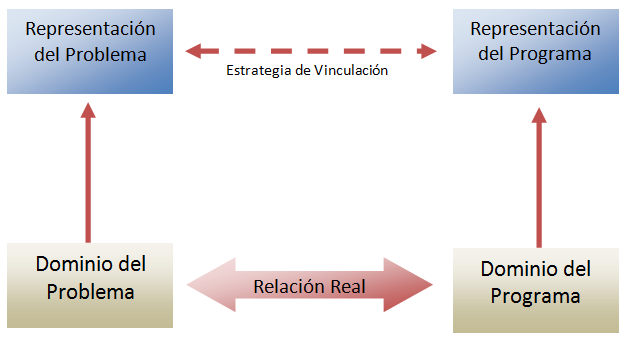
\includegraphics[scale= 0.7]{./dom.png}
}
\caption{Gráfico de Comprensión de Programas}
\end{figure} \label{captura1}

El inconveniente es que la relación real mostrada en la figura \ref{captura1}, es compleja de reconstruir, por ende se puede bosquejar una aproximación a través de los si\-guientes pasos: i) Elaborar una representación para el Dominio del Problema; ii)
Construir una representación del Dominio del Programa y iii) Elaborar un procedimiento de vinculación.
 
Para lograr con éxito los pasos antedichos se deben tener en cuenta conceptos muy importantes que son los cimientos sobre los cuales está sustentada la CP: los \textit{modelos cognitivos}, la \textit{extracción de información}, la \textit{administración de la información}, la \textit{visualización de software} y la \textit{interconexión de dominios}.

\section{Modelos Cognitivos}

Los \textit{Modelos Cognitivos} se refieren a las estrategias de estudio y las estructuras de información usadas por los programadores para comprender los programas. Estos modelos \cite{TIE89,VMAVA95,BROOK82,STOREY99} son importantes porque indican de que forma el programador comprende los sistemas y como incorpora nuevos conocimientos (aprende nuevos conceptos). 

Los modelos cognitivos están compuestos por: \textit{conocimientos}, \textit{modelos mentales} y \textit{procesos de asimilación} \cite{MBPHRU10}.

Existen 2 tipos de \textit{conocimientos} uno es el conocimiento interno el cual se refiere al conocimiento que el programador ya posee antes de analizar el código del sistema de estudio. Por otro lado existe el conocimiento externo que representa un soporte de información externo que le brinda al programador nuevos conceptos. Los ejemplos más comunes son la documentación del sistema, otros desarrolladores que conocen el dominio del problema, códigos de otros sistemas con similares características, entre otras tantas fuentes de información.

El concepto \textit{modelo mental} hace referencia a representaciones mentales que el programador elabora al momento de estudiar el código del sistema. 
%Estas representaciones mapean a distintas componentes del sistema. 
Algunos modelos construidos por los arquitectos de software como por ejemplo el diagrama de clases o el diagrama de casos de uso, entre otros pueden verse como representaciones visuales de modelos mentales. 

El \textit{proceso de asimilación} son las estrategias de aprendizaje que el programador usa para llevar adelante la comprensión de un programa. Los procesos de asimilación se pueden clasificar en tres grupos: Bottom-up, Top-Down e híbrida \cite{MPOB03,MAS05}.

El proceso de comprensión \textit{Bottom-up}, indica que el desarrollador primero lee el código del sistema. Luego, mentalmente las líneas de código leídas se agrupan en distintas abstracciones de más alto nivel. Estas abstracciones intermedias se van construyendo hasta lograr una abstracción comprensiva total del sistema.

Por otro lado, Brooks explica el proceso teórico \textit{top-down}, donde el programador primero elabora hipótesis generales del sistema en base a su conocimiento del mismo. En ese proceso se elaboran nuevas hipótesis las cuales se intentar validar y en ese proceso se generan nuevas hipótesis.
%Luego estas hipótesis generales son comprobadas y refinadas a nuevas hipótesis más detalladas. Estas hipótesis nuevas también son comprobadas y generan nuevas hipótesis.
Este proceso se repite hasta que se encuentre un trozo de código que implementa la funcionalidad deseada.

%Por otro lado el modelo de comprensión top-down es una estrategia en donde primero el programador usa el conocimiento adquirido del dominio del problema para construir perspectivas del sistema en forma de modelo y luego estas perspectivas se vinculen con los distintos fragmentos del código.

Para resumir, el proceso de aprendizaje bottom-up procede de lo más específico (código fuente) a lo más general (abstracciones). Mientras que el top-down es a la inversa.

Por último, el proceso \textit{híbrido} combina los dos conceptos mencionados top-down y bottom-up. Durante el proceso de aprendizaje del sistema, el programador combina libremente ambas políticas hasta llegar a comprender el sistema.

Para concluir sobre la temática de modelos cognitivos: el modelo mental es una representación mental que el programador tiene sobre el sector del sistema que esta analizando. Si esta representación se la vincula con los conocimientos que el propio programador posee, se logra un entendimiento de esa parte del sistema analizado, como así también incrementa los conocimientos del programador. Con esto se deja en claro la importancia de modelos cognitivos en el proceso de entendimiento de los sistemas.%CONSULTAR

\section{Extracción de Información}

En la ingeniería del software existe un área que se encarga de la \textit{extracción de la información}. Esta extracción se realiza en los sistemas de software y las técnicas utilizadas para tal fin se clasifican según el tipo de información que extraen. Existen dos tipos de informaciones: la Estática y la Dinámica.

La información estática está presente en los componentes del código fuente del sistema. Alguno de ellos son identificadores, procedimientos, comentarios, documentación.

Una estrategia para extraer la información estática consiste en utilizar técnicas tradicionales de compilación \cite{AHUL06}. Estas 
técnicas, utilizan un parser similar al empleado por un compilador. Este parser, por medio de acciones semánticas específicas procede a capturar elementos presentes en el código durante la fase de compilación. En la actualidad, existen muchas herramientas automáticas que ayudan a construir este tipo de parsers.

%Otra estrategia de extracción de información estática es la vista de grafo de llamadas a funciones\cite{MBPHRU10}. Las aristas de este grafo son funciones del programa de estudio y los arcos representan las llamadas entre dos funciones. Esta vista permite observar la invocación entre funciones. Utiliza la relación llamador-llamado en base solo al código fuente. Simplemente se colocan sentencias en el código indicando desde donde se invocan las funciones. Con esto se sabrá quien llama a una determinada función para llevar a cabo la construcción del grafo.

%Ambas estrategias estáticas descriptas no requieren ejecutar el sistema de estudio.

%Para construir el analizador se suele utilizar una herramienta automatizada que lee una gramática y después genera el parser. En esta gramática asociada a un lenguaje particular se insertan acciones semánticas que formarán parte del parser generado.
%Otra forma es usando grafo de llamadas a funciones en donde las aristas son funciones del programa de estudio y los arcos representan las llamadas entre dos funciones. A nivel conceptual es fácil de entender pero a veces la complejidad de los sistemas impiden una ágil realización sobre todo si los bloques de código tienen una complejidad temporal y espacial con cotas elevadas \cite{MBPHRU10}. Para la construcción de este grafo no se necesita ejecutar el programa.

Por otro lado, la información dinámica se basa en elementos del programa presentes durante una ejecución específica del sistema \cite{THBE99}. Una técnica encargada de extraer información dinámica es la instrumentación de código. Esta técnica inserta sentencias nuevas en el código fuente. La finalidad de las nuevas sentencias es registrar las actividades realizadas durante la ejecución del programa. 
%Para la extracción de este tipo de información se procede a bosquejar una técnica de instrumentación de código la cual consiste en insertar sentencias en el código sin modificar su semántica, así cuando el sistema se ejecute estas sentencias que contienen acciones se van a encargar de indicar que operaciones internas se llevaron a cabo para una determinada salida del programa.
Estas sentencias nuevas no modifican la funcionalidad original del sistema, por ende la inserción debe realizarse con sumo cuidado y de forma estratégica para no alterar el flujo normal de ejecución.

Como se explico en secciones precedentes, para extraer la información dinámica el sistema se debe ejecutar, mientras que no ocurre lo mismo a la hora de extraer la información estática.

La extracción de información cumple un rol fundamental en la CP. Como se explicó antes, en la CP se destaca la relación entre el dominio del problema y el dominio programa, como esta relación es compleja, se elabora una aproximación mediante el uso de representaciones (ver figura \ref{captura1}). Necesariamente, para poder bosquejar dichas representaciones se debe extraer información de ambos dominios.

Cabe destacar que extraer información de los sistemas implica tomar ciertos recaudos. Si la magnitud de información es demasiado grande se puede dificultar el acceso y el almacenamiento de la misma. Es por esto que se recurre a las técnicas de administración de información. En la próxima sección se explica con más detalles esta afirmación.

%Otra forma de extraer información dinámica, es usando un árbol de ejecución de funciones\cite{MBPHRU10}. Para armar esta estructura se necesita insertar sentencias en el código que señalen el inicio y fin de cada función. El orden en el que se ejecutan estas sentencias para una ejecución particular se resguardan en una pila, luego la pila es leída y el árbol se construye. Esta gráfica clarifica las llamadas que se hicieron entre funciones para una corrida particular.

%Los párrafos anteriores permiten percibir la importancia de las las técnicas de extracción de información estáticas y dinámicas. Sin estas técnicas sería imposible construir estrategias de comprensión de programas. Más precisamente, se necesitan para extraer información de los 2 dominios antedichos, el del problema y del programa (ver figura \ref{captura1}).

%Una vez extraída la información, la misma se recomienda que sea administrada.

%Volviendo al objetivo principal que es aproximarse en la construcción de relación del dominio del problema con el dominio programa a través de representaciones esta requiere la extracción de información de ambos dominios.

%La extracción de información del dominio del programa es una metodología sencilla de llevar a cabo por el hecho de que su extracción está claramente marcada. El inconveniente radica en la extracción de la información perteneciente al dominio del problema, porque esta información es sensible a las características propias de la aplicación. Para encarar este inconveniente la ingeniería del software propone tomar las fuentes de información informal las cuales pueden estar presentes en el código por ejemplo: comentarios, literales string; o fuera del mismo: documentación, entrevistas con el cliente etc. Un vez que se extraen estos componentes se les puede aplicar alguna técnica de análisis de información informal para interpretar algunas las funcionalidades de los componentes del sistema.

%Hasta aquí solo se ha mencionado estrategias de extracción información de los dominios del problema y del programa. Desafortunadamente el mapeo que relaciona la salida del sistema con los componentes que la integran queda a manos del programador y no abundan herramientas automatizadas que simplifiquen esta tarea.


\section{Administración de la Información}

Teniendo cuenta que lo sistemas son cada vez más amplios y complejos. El volumen de la información extraída de los sistemas crece notoriamente, por lo tanto se necesita administrar la información.

Las técnicas de administración de información se encargan de brindar estrategias de almacenamiento y acceso eficiente a la información recolectada de los sistemas. 

Dependiendo del tamaño de la información se utiliza una determinada estrategia. Estas estrategias indican el tipo de estructura de datos a utilizar y las operaciones de acceso sobre ellas \cite{AAJU88,TSTA80}. La eficiencia en espacio de almacenamiento y tiempo de acceso son claves a la hora de elegir una estrategia.

Cuando la cantidad de datos son de gran envergadura, se recomienda emplear una base de datos con índices adecuados para realizar las consultas \cite{ERNS99}.

Después que se administra la información, se recomienda  que la misma sea representada por alguna técnica de visualización. Esto permite esclarecer la información procesada del sistema al programador. El área encargada de llevar adelante esta tarea es la \textit{visualización de software}.

%Una temática importante en las técnicas explicadas SVS, BORS y SVSI es la visualización de software. En la siguiente sección se explica este punto.

\section{Visualización de Software}

La \textit{Visualización del Software} es una disciplina importante de la Ingeniería del Software. Esta disciplina, se encarga de visualizar la información presente en los programas, con el propósito de facilitar el análisis y la comprensión de los mismos. Esta cualidad es interesante ya que en la actualidad los sistemas son cada vez más amplios y complicados de entender.

La \textit{Visualización del Software} provee varias técnicas para implementar sistemas de visualización. Estos sistemas son herramientas útiles que se encargan de analizar los distintos módulos de un programa y generar vistas. Las vistas son una representación visual de la información contenida en el software. Esto permite, interpretar los programas de manera más clara y ágil. Dependiendo de la información que se desea visualizar existe una vista específica \cite{MPMR07}.%CONSULTAR

%De esta manera, facilita las arduas tareas de mantenimiento al programador sobre todo, en sistemas amplios y complicados. Este punto indica que la \textit{Visualización del Software} es un pilar importante para la CP.

%Las vistas cuando están bien construidas clarifican más la comprensión del sistema.


%Cabe recordar que la información concebida en un sistema puede ser estática o dinámica. 

%Existen distintos tipos de vistas, en si mismo, la primer vista de un sistema es el código en donde la información no está tan clara para un desarrollador ajeno sobre todo si el software es grande y complicado.

%Es por eso que se necesita recurrir a otras vistas que representen una abstracción mas clara del sistema.
 
%Las vistas poseen distintas características y para su construcción se requieren un conjunto de librerías gráficas. Dichas librerías son programas que simplifican la elaboración de las vistas y el diseñador de la visualización tiene la tarea de elegir que librería es la más adecuada para la vista que desea construir. Las librerías gráficas mas conocidas son Jung, Prefuse, Graphviz y Cairo \cite{BRM10}.

En la actualidad, existen distintos tipos de sistemas de visualización, algunos autores son: Myers, Price, Roman, Kenneth, Storey \cite{MBPHRU10}. Sin embargo, todos estos sistemas de visualización tienen algo en común, las vistas que son generadas por ellos representan conceptos situados solo en el dominio del programa, restando importancia al dominio del problema y a la relación entre ambos dominios.

Debido a esta falencia Berón \cite{MBPHRU10} propone variantes en los sistemas de visualización orientados a la CP. Estas variantes contemplan la representación visual de los conceptos en el dominio del problema, inclusive la visualización de la relación entre los dos dominios mencionados.

Para concluir, el objetivo primordial de la visualización de software orientada a la CP es generar vistas (representaciones visuales), que ayuden a reconstruir el vinculo entre el Dominio del Problema y el Dominio del Programa (figura \ref{captura1}). 


\section{Estrategias de Interconexión de \\Dominios}

Los conceptos explicados en los puntos anteriores como la \textit{visualización de software} y la \textit{extracción de la información} forman la base para armar estrategias de interrelación de dominios.

La \textit{Interconexión de Dominios} \cite{BRM10,MBPHRU10} en la Ingeniería del Software básicamente se atribuye a la transformación y vinculación del dominio de la aplicación de software (dominio del problema) con el dominio del programa (ver figura \ref{captura1}). Esta afirmación, como se explico en secciones anteriores es clave en la CP.

El objetivo es que cada componente de un dominio se vea reflejado en uno o más componentes de otro dominio y viceversa.%CONSULTAR

%Cuando se dice que relacionar el dominio del problema con el dominio del programa es importante ya que permite al desarrollador encontrar de forma mas ágil y rápida componentes en el software para una operación específica. Esto facilidad impacta directamente en los tiempos dedicados a la evolución y al mantenimiento del software por el simple hecho de que se reduce la ardua tarea que tiene el programador de comprender el código.
%Sin embargo, solo se podrá destacar este impacto si el software de estudio es muy amplio y complejo.

Un ejemplo de interconexión de dominios es cuando el dominio del código fuente de un programa, se puede transformar en un Grafo de Llamadas a Funciones (Dominio de Grafos). Cada nodo del grafo representa una función particular y cada arco las funciones que puede invocar. En este ejemplo la relación entre ambos dominios (código y grafo) es clara y directa. 

Es importante aclarar que existe una amplia gama de transformaciones entre dominios. La más escasa y difícil de conseguir es aquella que relaciona el Dominio del Problema con el Dominio del Programa (ver figura \ref{captura1}).

Sin embargo, actualmente existen técnicas recientemente elaboradas que conectan visualmente el dominio del problema y el dominio del programa usando la información estática y dinámica que se extrajo del sistema de estudio (ver figura \ref{captura1}). Como se dijo previamente, esta relación es de mucha importancia porque diagrama la salida del sistema y que elementos vinculados intervinieron.

Una de las técnicas es \textit{Simultaneous Visualization Strategy} SVS, esta se encarga de mostrar los distintos componentes de un programa en plena ejecución, mediante distintas vistas, usando un inspector de sentencias, de esta manera se obtiene una visualización cuando el sistema se está ejecutando. Esta estrategia usa un esquema de instrumentación de código, donde las acciones semánticas le van indicando a un visualizador la traza de invocaciones a funciones durante la ejecución del sistema \cite{BRM10,MPMR07,MBPHRU10}.

La otra estrategia se denomina \textit{Behavioral-Operational Relation Strategy} BORS, que a diferencia del SVS, espera a que termine la ejecución del sistema y luego la información recopilada por el instrumentador de código es procesada por BORS. Una vez procesada la información, BORS retorna una abstracción gráfica del código ejecutado. Un ejemplo de esta gráfica puede ser el Árbol de Ejecución de Funciones (ver sección anterior). BORS vincula los conceptos del código capturados en tiempo de ejecución con la información asociada al dominio del problema \cite{BRM10,MPMR07,MBPHRU10}.

Existe también, a nivel conceptual una técnica que combina ambas estrategias mencionadas llamada \textit{Simultaneous Visualization Strategy Improved} SVSI. Esta técnica disminuye los problemas que manifiestan tanto SVS como BORS y con ello se logra un mejor desempeño en cuanto a los resultados esperados \cite{BRM10,MPMR07,MBPHRU10}.

\section{Comentarios}

Para resumir las ideas tratadas en este capítulo, el área de la CP le da mucha importancia a la relación entre el Dominio del Problema y el Dominio del Programa. Esta relación ayuda al programador a entender con facilidad los programas ya que encuentra las partes del sistema que produjeron una determinada salida. Como es demasiado complicado este vínculo, se necesitan estudiar las temáticas pertinentes: los \textit{modelos cognitivos}, la \textit{extracción de información}, la \textit{administración de la información}, la \textit{visualización de software} y la \textit{interconexión de dominios}.

%llevan a cabo representaciones haciendo uso de la \textit{extracción de información} correspondiente a cada dominio. 

%Una vez construidas las representaciones de ambos dominios se procede a la elaboración de una estrategia de vinculación, el armado de esta estrategia se basa en los conceptos de \textit{interconexión de dominios}. Esta estrategia de vinculación ayuda al programador a entender con facilidad los programas ya que encuentra las partes del sistema que produjeron una determinada salida.

%Para facilitar la interconexión de dominios, se recomienda usar la \textit{Visualización del Software}. En esta área se elaboran determinadas vistas donde se puede materializar gráficamente las representaciones de los dominios y la estrategia de vinculación (ver figura \ref{captura1}). Estas vistas ayudan a armar un puente cognitivo entre los aspectos del sistema y los conocimientos del programador. Con esto el desarrollador logra una abstracción del sistema adecuada a su estructura mental.

Los conceptos antedichos son claves para la CP. También es importante la construcción de Herramientas de Comprensión de Sistemas. Estas herramientas presentan diferentes perspectivas del sistema facilitando su análisis y su inspección. Evitan que el programador invierta tiempo y esfuerzo en entender los módulos de los sistemas. De esta manera, se agilizan las tareas de evolución y mantenimiento del software.

En el próximo capítulo se presenta distintas estrategias de análisis que se basan en la extracción de información de los sistemas. El análisis puntual es sobre los identificadores presentes en el código. Algunas de ellas están implementadas en forma de Herramientas de CP.


%CAPITULO3=============================================================


\chapter{Análisis de Identificadores: Estado del Arte}

\lhead[]{CAPÍTULO 3. ANÁLISIS DE IDS: ESTADO DEL ARTE}

En el capítulo anterior se introdujo en el ámbito de comprensión de programas con las definiciones de los conceptos más importantes. Este capítulo se centra en el estado del arte de algunas técnicas y herramientas orientadas a la CP. Las mismas basan su análisis en los identificadores (ids) situados en los códigos de programas. También se explica de la importancia que tienen los comentarios y los literales al momento de examinar ids. Al final del capítulo se describe una conclusión sobre los temas tratados.

\section{Introducción}

Los equipos de desarrollos de software frecuentemente enfocan todo su esfuerzo en el análisis, diseño, implementación y mantenimiento de los sistemas, restándole importancia a la documentación. Por lo tanto, es común encontrar paquetes de software carentes de documentación, lo cual indica que la lectura de los códigos de los sistemas es la única manera de interpretarlos. Es necesaria la interpretación del sistema sobre todo en grandes equipos de desarrollo, por el simple hecho de que un integrante del equipo puede tomar código ajeno para continuar con su desarrollo o realizar algún tipo de mantenimiento.

Teniendo en cuenta que los códigos crecen con los nuevos requerimientos y el frecuente mantenimiento, los sistemas son más complejos y difíciles de entenderlos. He aquí la importancia del uso de las herramientas de comprensión, con ellas se puede lograr un entendimiento ágil y facilitar las arduas tareas de interpretación de códigos.

Como se mencionó en el capítulo anterior la CP brinda métodos, técnicas y herramientas que facilitan al programador entender los programas. Un aspecto importante de la CP es la extracción de información estática. Estas técnicas de extracción no necesitan ejecutar los programas para llevar a cabo la tarea. Una forma de implementarlas es aplicar técnicas de compilación conocidas para extraer información implícita detrás de los componentes visibles en los códigos.
%whats the name - Lawrie
Entre los distintos componentes visibles se conocen los ids y los comentarios como principal fuente de información para la CP. Sin embargo, cuando en el código no abundan los comentarios la única fuente importante son los ids. 

El la siguiente tabla se muestra un análisis léxico que se realizó sobre 2.7 millones de lineas de códigos escritos en lenguaje JAVA.

\begin{center}
	\begin{table}[h]
	
		\centering
   		\begin{tabular}{| l | c | c | c | c | }  
       
       \hline
  	   \textsf{Tipo} & \textsf{Cantidad} & \textsf{\%} & \textsf{Caracteres} & \textsf{\%} \\ \hline
  	   Palabras claves & 1321005 & 11.2 & 6367677 & 12.7 \\ \hline
   	   Delimitadores & 5477822 & 46.6 & 5477822 & 11.0 \\ \hline
       Operadores & 701607 & 6.0 & 889370 & 1.8 \\ \hline
       Literales & 378057 & 3.2 & 1520366 & 3.0 \\ \hline          
       \textbf{Identificadores} & 3886684 & 33.0 & \textbf{35723272} & \textbf{71.5} \\ \hline
       \textbf{Total} & \textbf{11765175} & \textbf{100.0} & \textbf{49978507} & \textbf{100.0} \\ \hline
     
   	\end{tabular}
   
	\label{tabla1}   
   \caption{Resultado del Análisis Léxico}
   
  \end{table} 
\end{center}

\vspace{-2.5em}

En la tabla \ref{tabla1} se ve claramente que más de las dos terceras partes (71.5\%) de los caracteres en el código fuente forman parte de un id \cite{DFPM05,DMDJ13}. 
Por ende, en el ámbito de CP los ids son una fuente importante de información que el lector del código o encargado de mantenimiento debe tener en cuenta. Utilizar una herramienta que analice los ids dando a conocer su significado ayuda a revelar esta información, mejora la comprensión, aumenta la productividad y agiliza el mantenimiento de los sistemas.

Por lo antedicho, construir herramientas de CP que analicen ids en los códigos fuentes de los programas constituye un aporte importante al ámbito de CP. Antes de comenzar con la incursión de herramientas existentes que analizan ids, se detallan algunos conceptos claves relacionados.

\section{Conceptos claves}

\textit{“Un \textbf{Identificador (id)}: básicamente se define como una secuencia de letras, dígitos o caracteres especiales de cualquier longitud que sirve para identificar las entidades del programa”}
 
Cada lenguaje tiene sus propias reglas que definen como pueden estar construidos los nombres de sus ids. Por ejemplo, en JAVA no está permitido declarar ids que coincidan con palabras reservadas o que contengan operadores relacionales o matemáticos ($+$ $-$ $\&$ $!$ $\%$), a excepción del guión bajo (\_ ) o signo peso (\$). Ejemplo: \textsf{var\_char, var\$char}.

Generalmente, la buena practica de programación recomienda que un id dentro del código este asociado a un concepto del programa. 

\begin{center}
\textsf{Identificador $\Leftrightarrow$ Concepto}
\end{center}

Dicho de otra manera un id es un representante de un concepto ubicado en el dominio del problema \cite{DFPM05,DMDJ13} (ver capítulo 2). Por ejemplo, el id \textsf{openWindow} está asociado al concepto `abrir una ventana'.

%whats the name - Lawrie
%Para mejorar la CP se requiere que los nombres de los ids comuniquen de manera clara los conceptos que representan. Sin embargo, en la práctica no se tiene muy en cuenta. 

Uno los requisitos importantes que debe reunir un programa para facilitar su comprensión es que sus ids sean claros. Sin embargo, dicho requerimiento no es tenido en muy en cuenta por los programadores \cite{DFPM05,DLHD06,DCHD06}.

En la siguiente sección se menciona como la semántica de los ids impacta enormemente en la lectura comprensiva de los conceptos asociados y por ende también afecta a la CP.

\pagebreak
\section{Nombramiento de Identificadores}

%Deißenbock and Pizka DFPM05
%Intro
Durante los desarrollos de los sistemas, las reglas de construcción de ids se enfocan más en el formato del código y el formato de la documentación, en lugar de enfocarse en el concepto que el id representa. 

Un etapa importante en la vida de los sistemas es el mantenimiento (ver capítulo 2), generalmente el encargado de hacerlo no tiene en cuenta los nombres de los ids para interpretar el código.

%También durante la etapa de mantenimiento del software la forma en la que los ids están nombrados no es muy tenida en cuenta para comprender el sistema. 

Antes de proseguir sobre la importancia del nombramiento, a continuación se clasifican las distintas formas que se puede nombrar un id.

\subsection{Clasificación}
Estudios realizados con 100 programadores \cite{DCHD06} sobre comprensión de ids indican que existen tres formas principales de construir (tomando como ejemplo el concepto \textsf{File System Input}): 

\begin{itemize}
\itemsep0em%reduce espacio
\item Palabras completas (\textsf{fileSystemInput}).
\item Abreviaciones (\textsf{flSysIpt}).
\item Una sola letra\footnote[1]{Este nombramiento lo llaman acrónimo algunos autores.} (\textsf{fsi}). 
\end{itemize}

De más está decir que los nombres de los ids pueden estar compuestos por más de una palabra como se describió en los ítems anteriores.

Los estudios antedichos arrojaron que las palabras completas son las más comprendidas, sin embargo las estadísticas marcan en algunos casos que las abreviaciones que se ubican en segundo lugar, no demuestran una diferencia notoria con respecto a las palabras completas \cite{DCHD06}.

Los investigadores Feild, Binkley, Lawrie \cite{FBL06,HDD06,DMDJ13}, clasifican los nombres de los ids con 2 términos conocidos en la jerga del análisis de ids: \textit{hardwords} y \textit{softwords}.

Los \textit{hardwords} destacan la separación de cada palabra que compone el identificador a través de una marca específica; algunos ejemplos son: \mbox{\textsf{fileSystem}}\footnote[2]{Este nombramiento lo suelen llamar camel-case.} marca bien la separación de cada palabra con el uso de mayúscula entre las minúsculas o \mbox{\textsf{fileSYSTEM}} así también como utilizar un símbolo especial como es el caso del guión bajo \textsf{file\_system}. 

En cambio los \textit{softwords} no poseen ningún tipo de separador o marca que de indicios de las palabras que lo componen; por ejemplo: \textsf{textinput} o \textsf{TEXTINPUT} se compone por \textsf{text} y por \textsf{input} sin tener una marca que destaque la separación.

La nomenclatura de \textit{hardwords} y \textit{softwords} se utilizará en el resto de este trabajo final. En la próxima sección se destacan afirmaciones sobre la importancia de los nombres utilizados en los ids.

%Si bien en el párrafo anterior se dio una taxonomía de como se clasifican los ids, en los ejemplos no se refleja como normalmente se nombra un id.
%Generalmente los programadores para reducir el esfuerzo de tipeo escriben los ids en forma abreviada compuestos por mas de una palabra, esto se lo conoce con el nombre de acrónimos. Para dar un ejemplo sobre esto: el id \textsf{fileSystem} los programadores lo suelen nombran como \textsf{flSys}, \textsf{fiStm}, \textsf{fl\_sys} u otras tantas posibles representaciones abreviadas.

%Caprile and Tonella state that “identifier names are one of the most important sources of information about program entities”\cite{BCPT00}

%Caprile and Tonella - Software entities are born and live with their names. \cite{BCPT99}

\begin{figure}[t] %[h] para here [b] para bottom [t] para top
\centering
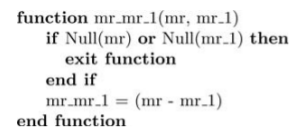
\includegraphics[scale= 0.70]{./idd_1.png}
\caption{Trozo de Código de un Sistema Comercial}
\label{captura2}
\end{figure} 

%================================
\subsection{Importancia del Nombramiento}
En la actualidad existen innumerables convenciones en cuanto a la construcción sintáctica de los ids, alguno de ellos son:

\begin{itemize}
\itemsep0em%reduce espacio
\item En el caso de JAVA, los nombres de los paquetes deben ser con minúscula (main.packed). Las clases con mayúscula en la primer letra de cada palabra que compone el nombre (MainClass).

\item En el caso de C\#, las clases se nombran igual que JAVA. Pero para el caso de los paquetes deben comenzar con mayúscula y el resto minúscula (Main.Packed).
\end{itemize}

Esto indica que se concentra más en los aspectos sintácticos del id y no tanto en los aspectos semánticos en lo que respecta al nombramiento. 

%Las investigaciones realizadas por Deissenboeck y Pizka \cite{DFPM05} a este problema parte de que cada nombre de id está asociado a un concepto del dominio del problema y viceversa. 
%Mas formalmente se puede ver como una función biyectiva:

%\begin{center}
%\textsf{Nombre $\Leftrightarrow$ Concepto}
%\end{center} 

%En este contexto se dice que se logra un nombramiento conciso y consistente de ids.



%Problema: de porque no existe un correcto nombramiento
Una evidencia fehaciente de la importancia en el nombramiento semántico son las técnicas que se aplican para protección de código. Algunas de ellas se encargan de reemplazar los nombres originales de los ids por secuencias de caracteres aleatorios y de esta manera se reduce la comprensión. Estas técnicas se conocen con el nombre de ofuscación de código. La ofuscación es común en los sistemas de índole comercial, en la figura \ref{captura2} se puede observar un ejemplo tomado de un caso real, en donde la función \textsf{mr\_mr\_1} no parece complicada pero se desconoce la finalidad de su ejecución \cite{DFPM05}.

A su vez, los programadores cuando desarrollan sus aplicaciones, restan importancia al correcto nombramiento semántico de los ids. Existen tres razones destacadas que conllevan a esto:

\begin{enumerate}
\itemsep0em%reduce espacio
\item Los ids son escogidos por los programadores, sin tener en cuenta los conceptos que tienen asociados.

\item Los desarrolladores tienen poco conocimiento de los nombres usados en  ids ubicados en otros sectores del código fuente.

\item Durante la evolución del sistema, los nombres de los ids se mantienen y no se adaptan a nuevas funcionalidades (o conceptos) que puedan tener asociado.
\end{enumerate}

En este sentido, el mal nombramiento de los ids se combate con la programación “menos egoísta”. Esta consiste en hacer programas más claros y entendibles para el futuro lector que no está familiarizado con el código. Para lograrlo se deben respetar dos reglas en cuanto al nombramiento \cite{DFPM05,DLHD06}:

%\noindent remueve la sangria!
\begin{framed}
\noindent \textbf{Nombramiento Conciso:} El nombre de un id es conciso, si la semántica del nombre coincide exactamente con la semántica del concepto que el id representa.

\noindent \textbf{Nombramiento  Consistente:} Para cada id, debe tener asociado si y solo si, un único concepto.
\end{framed}

Un ejemplo de conciso es \textsf{output\_file\_name} que representa el concepto de `nombre de archivo de salida', distinto es el nombre \textsf{file\_name}, el cual no representa de forma semánticamente concisa el concepto mencionado.

%sinonimos y homonimos
Los propiedades que violan el nombramiento consistente en los ids son conocidos en el lenguaje natural con el nombre de sinónimos y homónimos. 

Los homónimos son palabras que pueden tener más de un significado. Por ende, si el nombre de un id esta asociado a más de un concepto, no estará claro que concepto representa. Por ejemplo, un id con el nombre \textsf{file} generalmente se asocia al concepto de `archivo', pero puede que se refiera a una estructura del tipo cola o a una fila en una tabla.

Por otro lado, los sinónimos indican que para un mismo concepto pueden tener asociados diferentes nombres. Por ejemplo, un id con el nombre \mbox{\textsf{accountBankNumber}} y otro \textsf{accountBankNum} son sinónimos porque hacen referencia al mismo concepto `número de cuenta bancaria'. 

Esta demostrado \cite{DFPM05,DLHD06,DMDJ13} que la ausencia de nombramiento consistente tales como se menciono anteriormente, hacen que se dificulte identificar con claridad los conceptos en el dominio del problema, lo que hace aumentar los esfuerzos de comprensión del programa. 


Por lo tanto, si los ids están nombrados de forma concisa (identificando bien al concepto) y la consistencia está presente, se pueden descubrir los conceptos que representan en el dominio del problema más fácilmente. De esta manera, se agiliza la comprensión, aumenta la productividad, mejora la calidad durante la etapa de mantenimiento \cite{DFPM05,DLHD06}.%agregar mas bibliografia

Intuitivamente, se necesita que los ids representen bien al concepto, ya que mayor será impacto que tendrá en la interpretación del sistema \cite{DFPM05,DLHD06}.Sin embargo, durante las etapas de desarrollo y mantenimiento del software, es muy difícil mantener una consistencia global de nombres en los ids, sobre todo si el sistema es grande. Cada vez que un concepto se modifica el nombre del id asociado debe cambiar y adaptarse a la modificación.

%solucion propuesta
Los autores Deissenboeck y Pizka \cite{DFPM05} proponen utilizar una herramienta que solucione los problemas de mal nombramiento planteados anteriormente. Dada la dificultad que conlleva construir una herramienta totalmente automática que se encargue de nombrar correctamente los ids, ellos elaboraron una herramienta semi-automática que necesita la intervención del programador. Esta herramienta, a medida que el sistema se va desarrollando, construye y mantiene un diccionario de datos compuesto con información de ids. En el ámbito de la ingeniería del software el concepto de diccionarios de datos es importante.


\begin{verse}
\textbf{Diccionarios de Datos:} Este concepto conocido también como `glosario de proyecto' se recomienda en los textos orientados a la administración de proyectos de software. Con los diccionarios se describe en forma clara todos los términos utilizados en los grandes sistemas de software. También brindan una referencia completa a todos los participantes de un proyecto durante todo el ciclo de vida del producto.
\end{verse}

Este concepto sirvió de inspiración a los autores para construir la herramienta. A continuación se la describe. \\ \\

\begin{figure}[h] %[h] para here [b] para bottom [t] para top
\centerline{%queda centrada mejor la imagen
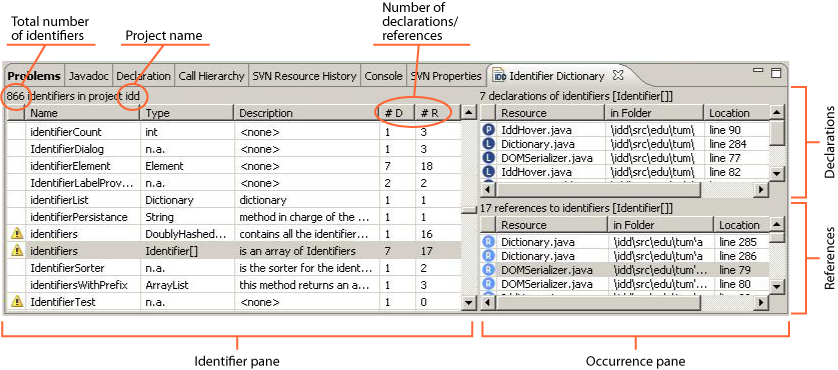
\includegraphics[scale= 0.55]{./idd_2.png}
}
\caption{Visualización de Identifier Dictionary}
\label{captura3}
\end{figure}
\pagebreak
\subsection{Herramienta: Identifier Dictionary}

La herramienta conocida con el nombre de \textit{Identifier Dictionary} (IDD)\footnote[1]{http://www4.informatik.tu-muenchen.de/\~{}ccsm/idd/index.html} construida por Deissenboeck y Pizka \cite{DFPM05} actúa como un diccionario de datos que ayuda al desarrollador a mantener la consistencia de nombres en los ids de un proyecto JAVA. Es una base de datos que almacena información de los ids tales como el nombre, el tipo del objeto que identifica y una descripción comprensiva.

La herramienta IDD ayuda a reducir la creación de nombres sinónimos y asiste a escoger un nombre adecuado para los ids siguiendo el patrón de nombres existentes. Aumenta la velocidad de comprensión del código en base a las descripciones de cada id. El equipo encargado de tareas de mantenimiento localiza un componente del dominio del problema y luego su correspondiente id de manera ágil. Otro aporte que hace la herramienta es asegurar la calidad de los nombres (nombres concisos) de los ids con un esfuerzo moderado, usando como ayuda la descripción comprensiva ubicada en la base de datos \cite{DFPM05,LFBEX07}.

Se implementó como extensión de la IDE Eclipse 3.1\footnote[2]{http://www.eclipse.org/jdt}. Se visualiza en el panel de las vistas de la IDE y consiste de tres secciones (Figura \ref{captura3}):

\begin{figure}[t] %[h] para here [b] para bottom [t] para top
\centerline{%queda centrada mejor la imagen
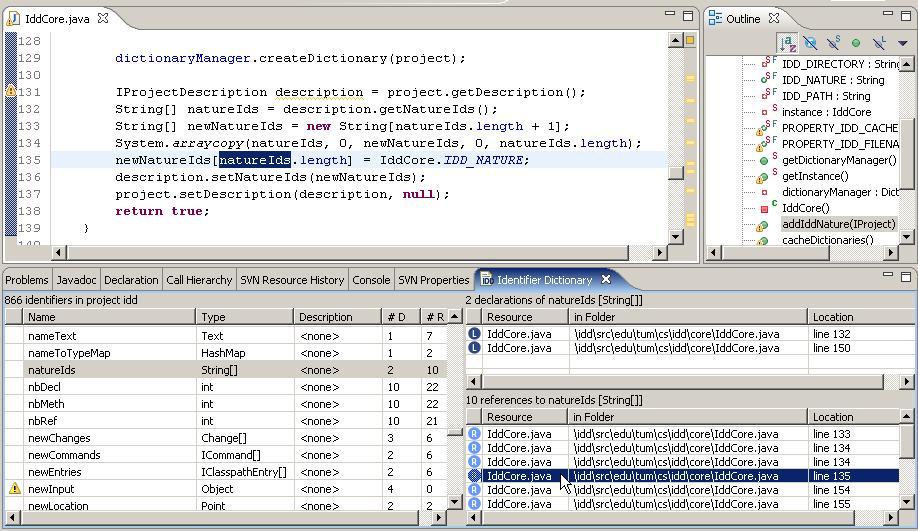
\includegraphics[scale= 0.50]{./idd_3.png}
}
\caption{Visualización de Identifier Dictionary}
\label{captura4}
\end{figure} 

\begin{itemize}
\itemsep0em%reduce espacio
\item Una tabla con información de los ids en el proyecto: nombre, tipo, descripción, cantidad de declaraciones y cantidad de referencias (Identifier pane).
\item Una lista de Ids declarados en el proyecto (Ocurrence pane).
\item Una lista de referencias de los ids en el proyecto (Ocurrence pane).
\end{itemize}

Mientras se realiza el desarrollo del código la herramienta asiste al programador a llevar un buen nombramiento en los ids, a través de las siguientes características:

\textbf{Navegación en el código fuente:} Si se selecciona un id en la tabla de ids (inferior izquierda), mostrará la ubicación exacta en donde se encuentra cada declaración y referencia (Figura \ref{captura4}).


%\begin{figure}[h] %[h] para here [b] para bottom [t] para top
%\centering
%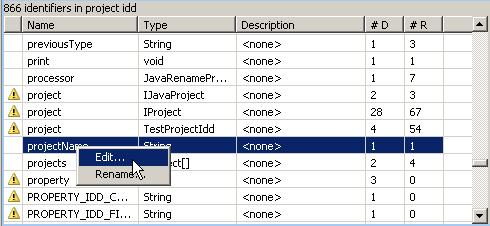
\includegraphics[scale= 0.55]{./idd_4.png}
%\caption{Visualización de Identifier Dictionary}
%\label{captura5}
%\end{figure}
%
%\textbf{Guardar descripción:} Botón derecho en el panel de ids y luego en edit. Permite agregar una descripción comprensiva (Figura \ref{captura5}).

%\begin{figure}[h] %[h] para here [b] para bottom [t] para top
%\centering
%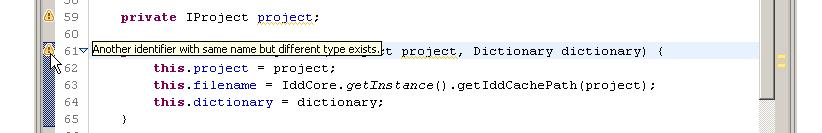
\includegraphics[scale= 0.55]{./idd_5.png}
%\caption{Visualización de Identifier Dictionary}
%\label{captura6}
%\end{figure}
\begin{figure}[t] %[h] para here [b] para bottom [t] para top
\centerline{%queda centrada mejor la imagen
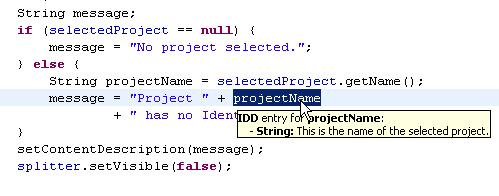
\includegraphics[scale= 0.70]{./idd_7.png}
}
\caption{Visualización de Identifier Dictionary}
\label{captura8}
\end{figure}

\textbf{Advertencias (warnings):} Mientras se realiza la recolección de ids los íconos de advertencia indican potenciales problemas en el nombramiento.  Los dos tipos de mensajes que se muestran son: dos ids con el mismo nombre pero distinto tipos y el id es declarado pero no referenciado\footnote[1]{Similar a los warnings de Eclipse}.


%\begin{figure}[h] %[h] para here [b] para bottom [t] para top
%\centering
%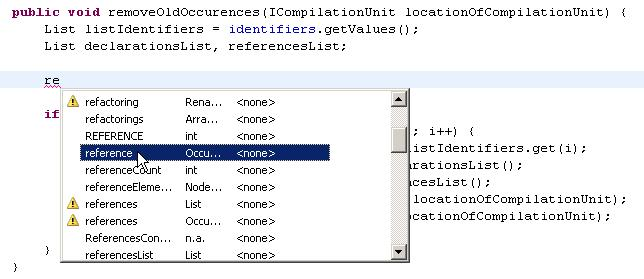
\includegraphics[scale= 0.55]{./idd_6.png}
%\caption{Visualización de Identifier Dictionary}
%\label{captura7}
%\end{figure}

\textbf{Mensajes pop-up:} Se puede visualizar información tales como la descripción del id posicionando el cursor sobre el id en el código fuente mientras se está programando (Figura \ref{captura8}).

\textbf{Auto-completar nombres:} Las IDE\footnote[2]{Entornos de desarrollos integrados, por su siglas en inglés. Netbeans, Eclipce etc.} actuales proveen la función de auto-completar.
Sin embargo, esta funcionalidad falla cuando los nombres de los ids no están declarados dentro del alcance actual de edición. Con el plugin IDD a la hora de auto-completar mira todos los ids del proyecto sin importar el ambiente en el que se encuentre.\\

\textbf{Renombre global de ids:} Esta función permite renombrar cualquier id generando una vista previa y validando el nombre de los ids a medida que sistema va evolucionando. De esta forma se preserva la consistencia global de nombres.

La herramienta IDD trabaja internamente con un colector de ids que está acoplado al proceso de compilación del proyecto (Build Proyect) de Eclipse. Los ids se van recolectando a medida que el programa se va compilando. Los nombres, el tipo, la descripción se van guardando en un archivo XML. También se puede exportar en un archivo en formato HTML el cual permite una lectura más clara de los ids con toda información asociada \cite{DFPM05}.


%%=========Lawrie

La herramienta IDD colabora en mejorar el nombramiento de los ids con un esfuerzo moderado como se describió antes. 

Sin embargo, los investigadores Feild, Binkley, Lawrie \cite{LFBEX07,DLHD06} determinaron que los esfuerzos son moderados solo para sistemas que se empiezan a programar desde el comienzo y no con sistemas ya existentes.

Para concluir con esta sección, la buena calidad en el nombramiento de los ids descripta mejora el entendimiento del código. En este sentido, muchos expertos sostienen que las técnicas de Ingeniería Inversa se emplean con mayor precisión si el código esta bien escrito. Algunas de estas técnicas que tiene como objetivo mejorar la CP se encargan de traducir los nombres abreviados de los ids a palabras más completas en lenguaje natural. En la sección siguiente se describen este tipo de técnicas de regresión.

%%=====================================
\pagebreak
\section{Traducción de Identificadores}

Los lectores de códigos de programas tienen inconvenientes para entender el propósito de los ids y deben invertir tiempo en analizar el significado de su presencia. Por esta razón, las estrategias automáticas dedicadas a facilitar este análisis son bienvenidas en el contexto de la CP.

Para aliviar el inconveniente mencionado anteriormente, se debe descubrir la información que ocultan los ids detrás de sus abreviaturas. Esta información es relevante ya que pertenece al dominio del problema \cite{EHPV09,LFBEX07}. 

\subsection{Conceptos y Desafíos observados}

Una manera de descubrir la información oculta detrás de los ids es intentar convertir estas abreviaturas en palabras completas del lenguaje natural. Por ende, el foco del análisis de los ids se basa en la traducción de palabras abreviadas a palabras completas.

El proceso automático que se lleva a cabo para realizar la traducción de ids consta de dos pasos \cite{LFBEX07}:

\begin{enumerate}
\itemsep0em%reduce espacio
\item \textbf{División:} Separar el id en las palabras que lo componen usando algún separador especial\footnote[1]{Siempre y cuando el id contenga más de una palabra.}. (Ejemplo: \textsf{flSys} $\Rightarrow$ \textsf{fl-sys}).

\item \textbf{Expansión:} Expandir las abreviaturas que resultaron como producto del paso anterior. (Ejemplo: \textsf{fl-sys} $\Rightarrow$ \textsf{file system}).
\end{enumerate}

Cabe mencionar que el ejemplo mostrado en ambos pasos corresponde a un caso de \textit{hardword} (ver sección anterior) en donde la separación de las palabras es destacada. Sin embargo, la dificultad se presenta en los \textit{softwords} (ver sección anterior) ya que la división no está marcada (Ejemplo: \textsf{hashtable} $\Rightarrow$ \textsf{hash-table}). Existen también casos híbridos (Ejemplo: \textsf{hashtable\_entry}). En este caso el id tiene una marca de separación (guión bajo) con dos hardwords \textsf{hashtable} y \textsf{entry}. A su vez el hardword \textsf{hashtable} posee dos softwords \textsf{hash} y \textsf{table}, mientras que \textsf{entry} es un hardword compuesto por un único softword. 

%noindent - Elimina sangria
\begin{framed}
\noindent El objetivo primordial y más difícil en la traducción de ids es detectar los casos de softword. Luego proceder a separar las palabras abreviadas que la componen para posteriormente realizar la expansión \cite{FBL06,LFBEX07}.  
\end{framed}

Para afrontar este objetivo los especialistas deciden recurrir a fuentes de palabras en lenguaje natural (inglés en este caso). Existen 2 tipos de fuentes, dentro del mismo código extrayendo palabras presentes en comentarios, literales y documentación. La otra fuente se encuentra fuera del programa consultando diccionarios o listas de palabras predefinidas. 

Habiendo explicado el proceso encargado de expandir las abreviaturas de un id a palabras completas, el siguiente paso es describir las herramientas conocidas que lo implementan. 

La autora Emily Hill \cite{EZH08} con alto reconocimiento por su investigación en lo que respecta a expandir ids en códigos java, explica algunas amenazas y desafíos a tener en cuenta a la hora de desarrollar herramientas que analizan ids. A continuación se explican algunas de ellas.

\begin{description}
\itemsep0em%reduceenglish espacio
\item[Dificultad para armar diccionarios apropiados:]  La mayoría de los diccionarios en Inglés se usan para corregir la ortografía. Las palabras que incluyen son sustantivos propios, abreviaciones, contracciones\footnote[1]{Palabras en inglés que llevan apostrofes, ejemplo: let's.} y demás palabras que puedan aparecer en un software. Sin embargo, la inclusión de muchas palabras genera que una simple abreviación ($char,tab,id$) se trate como una palabra expandida y no se expanda. Por el contrario, si el diccionario contiene pocas palabras, la expansión se realiza más frecuente de lo normal.
% lo ideal es disponer de un diccionario con palabras que incluyan solo palabras adecuadas al ámbito de la ciencias de la computación pero lamentablemente esto no está disponible.

\item[Las abreviaciones poseen muchos candidatos a expandir:] Es complicado para un id abreviado con \textsf{def} determinar con precisión cual es la mejor traducción entre tantos candidatos \textsf{definition, default, defect}. Otra observación hecha, es que mientras más corta es la abreviación más candidatos posee, el ejemplo más común es \textsf{i} que generalmente es \textsf{integer} pero podrían ser otros \textsf{interface, interrupt}, etc. Se requieren procesos inteligentes para solucionarlo.
\pagebreak
\item[El tipo de la abreviación afecta el número de candidatos:] Si la abreviatura se mira como prefijo tiene menos candidatos a traducirse, un ejemplo es \textsf{str} el cual tiene \textsf{string, stream}. En cambio si las letras de \textsf{str} forman parte de la palabra tiene más posibilidades de expansión S\textsf{ubs}TR\textsf{ing}, ST\textsf{o}R\textsf{e}, S\textbf{ep}T\textbf{embe}R, S\textbf{a}T\textbf{u}R\textbf{n}.
\end{description}


Las palabras abreviadas, usadas en los ids dependen mucho de la idiosincrasia del programador. Por lo tanto construir herramientas automáticas que analicen ids representa un verdadero desafío en el área de CP.

En las próximas 2 secciones se explican algoritmos encargados de la división de ids, y en la secciones subsiguientes se describen algoritmos de expansión.

%Se puede usar técnicas de recuperación de información para mejorar el procedimiento de traducción.

%greedy - samurai 
\subsection{Algoritmo de División: Greedy}

El algoritmo Greedy elaborado por Lawrie, Feild, Binkley \cite{DLFB06,FBL06,HDD06,LFBEX07,EHPV09} divide las palabras que forman parte de un id, es sencillo y emplea tres listas:
\begin{description}
\itemsep0em%reduce espacio
\item[Palabras de diccionarios:] Contiene palabras de diccionarios públicos y del diccionario que utiliza el comando de Linux \textsf{ispell}\footnote[1]{Comando de Linux generalmente utilizado para corregir errores ortográficos (inglés) en archivos de texto. http://linuxcommand.org/man\_pages/ispell1.html}.

\item[Abreviaciones conocidas:] La lista se arma con abreviaciones extraídas de distintos programas y de autores expertos. Se incluyen abreviaciones comunes (ejemplo: \textsf{alt} $\rightarrow$ \textsf{altitude}) y abreviaciones de programación \mbox{(ejemplo: \textsf{txt} $\rightarrow$ \textsf{text}).}

\item[Palabras excluyentes (stop list):] Posee palabras que son irrelevantes para realizar la división de los ids. Incluye palabras claves (ejemplo: \texttt{while}), ids predefinidos (ejemplo: \texttt{NULL}), nombres y funciones de librerías (ejemplo: \texttt{strcpy},\texttt{errno}), y todos los ids que puedan tener un solo caracter. Esta lista es muy grande.
\end{description}

El algoritmo de Greedy utiliza las 3 listas nombradas al comienzo de la sección en forma de variable global. Esto ocurre porque las 3 listas son usadas por subrutinas más tarde. El algoritmo procede de la siguiente manera (ver algoritmo \ref{GSA}), el id que recibe como entrada primero se divide (con espacios en blanco) en las hardwords que lo componen (ejemplo: \textsf{fileinput\_txt} $\rightarrow$ \mbox{\textsf{fileinput}} y \textsf{txt} en la línea 2, si es camelcase \textsf{fileinputTxt} $\rightarrow$ \textsf{fileinput} y \textsf{txt} en la línea 3). Luego, cada palabra resultante en caso que esté en alguna de las 3 listas, se distingue como un único softword (ejemplo: \textsf{txt} pertenence a la lista de abreviaciones conocidas - línea 5). Si alguna palabra no está en alguna lista se considera como múltiples softwords que necesitan subdividirse (ejemplo: \textsf{fileinput} $\rightarrow$ \textsf{file} y \textsf{input} - línea 5).
Para subdividir estas palabras se buscan los prefijos y los sufijos más largos posibles dentro de ellas. Esta búsqueda también se realiza utilizando las 3 listas antes mencionada (líneas 6 y 7).

Por un lado se buscan prefijos con un proceso recursivo (ver Función \mbox{\textbf{buscarPrefijo}}). Este proceso comienza analizando toda la palabra por completo. Se van extrayendo caracteres del final hasta encontrar el prefijo más largo o no haya más caracteres (líneas 5 - 7 de la función). %Lo siguiente hay que chequiarlo con Mario
Cuando una palabra se encuentra en alguna lista (línea 3 de la función) se coloca un separador (` '). El resto que fue descartado se procesa por \textbf{buscarPrefijo} para buscar más subdivisiones (línea 4).

De manera simétrica, otro proceso recursivo se hace cargo de los sufijos (ver Función \textbf{buscarSufijo}). También extrae caracteres, pero en este caso desde la primer posición hasta encontrar el sufijo más largo presente en alguna lista o no haya más caracteres (líneas 5 - 7 de la función). %Lo siguiente hay que chequiarlo con Mario
De la misma forma que la función de prefijos cuando encuentra una palabra, se inserta un separador (` ') y el resto se procesa por la función \textbf{buscarSufijo} (línea 4).

Una vez que ambos procesos terminaron, los resultados (\textsf{resultadoPrefijo, resultadoSufijo}) son retornados al algoritmo principal (líneas 6 y 7). Mediante una función de comparación se elije el que obtuvo mayores particiones (línea 8). Finalmente, el algoritmo Greedy retorna el id destacando las palabras que lo componen mediante el separador espacio \mbox{(\textsf{file input txt})}.

La ventaja de hacer dos búsquedas (prefijo y sufijo) radica en aumentar las chances de dividir al id. A modo de ejemplo, suponiendo que la palabra abreviada \textsf{fl}
no se encuentra en ninguno de los 3 listados y las palabras \textsf{input} y \textsf{txt} si están. Dada esta situación, si el id \textsf{flinputtxt} se procesa por ambas rutinas, el resultado será que \textbf{buscarPrefijo} no divida al id. Esto sucede porque al retirar caracteres del último lugar nunca se encontrará un prefijo conocido. Más precisamente al no dividirse entre \textsf{fl} e \textsf{input} el resto de la cadena no se procesará y tampoco se dividirá entre \textsf{input} y \textsf{txt}. 

Sin embargo, este inconveniente no lo tendrá \textbf{buscarSufijo} porque al retirar los caracteres del principio de la palabra, \textsf{input txt} será separado. Como \textsf{input} es una palabra conocida se agregará un espacio entre \textsf{fl input}. De esta manera el id queda correctamente separado \textsf{fl input txt}.\\


\begin{algorithm}[H]%H fuerza que se genere aqui
\LinesNumbered%enumera las lineas
\SetKwInOut{Input}{Entrada}\SetKwInOut{Output}{Salida}
\SetKwInOut{Global}{Var Global}
\Global{\textit{\textbf{ispellList}} \tcp{\textit{Palabras de ispell + Diccionario}}}
\Global{\textit{\textbf{abrevList}} \tcp{\textit{Abreviaciones conocidas}}}
\Global{\textit{\textbf{stopList}} \tcp{\textit{Palabras Excluyentes}}}
\Input{\textit{\textbf{idHarword}} \tcp{\textit{identificador a dividir}}}
\Output{\texttt{softwordDiv} \tcp{\textit{id separado con espacios}}}

\BlankLine
\texttt{softwordDiv} $\leftarrow$ “”

\texttt{softwordDiv} $\leftarrow$ dividirCaracteresEspecialesDigitos(\textit{\textbf{idHarword}})

\texttt{softwordDiv} $\leftarrow$ dividirCamelCase(\texttt{softwordDiv})

\BlankLine
\ForAll{$($Para cada substring \textit{\textbf{s}} separado por ` ' en \texttt{softwordDiv}$)$}{
\BlankLine

\If{$($\textbf{s} no pertenece a $($\textit{\textbf{stopList}} $\cup$ \textit{\textbf{abrevList}} $\cup$ \textbf{ispellList} $))$}{
\BlankLine
sPrefijo $\leftarrow$ buscarPrefijo(\textit{\textbf{s}},“”)

sSufijo $\leftarrow$ buscarSufijo(\textit{\textbf{s}},“”)
\BlankLine
\tcp{\textit{Se elije la división que mayor particiones hizo.}}
\textit{\textbf{s}} $\leftarrow$ maxDivisión(sPrefijo,sSufijo)

}
}
\BlankLine
\Return \texttt{softwordDiv} \tcp{\textit{Retorna el id dividido por espacios.}}

\caption{División Greedy\label{GSA}}
\end{algorithm}

\begin{function}[H]
\LinesNumbered%enumera las lineas
\SetKwInOut{Input}{Entrada}\SetKwInOut{Output}{Salida}
\Input{\textit{\textbf{s}} \tcp{\textit{Abreviaturas a dividir}}}
\Output{\textit{\textbf{abrevSeparada}} \tcp{\textit{Abreviaturas separadas}}}
\BlankLine
\tcp{\textit{Punto de parada de la recursión.}}
\If{$($length$($\textit{\textbf{s}}$)$ $=$ 0$)$}{
\BlankLine
\Return \textit{\textbf{abrevSeparada}}
}
\BlankLine
\If{$($\textbf{s} pertenece a $($\textit{\textbf{stopList}} $\cup$ \textit{\textbf{abrevList}} $\cup$ \textbf{ispellList} $))$}{
\BlankLine
%\tcp{\textit{Se separa con espacio y se ejecuta la función con el resto.}}
\BlankLine
\Return (\textit{\textbf{s}} $+$ ` ' $+$ buscarPrefjjo(\textit{\textbf{abrevSeparada}},“”) )
}
\BlankLine
\tcp{\textit{Se extrae y se guarda el último caracter de s.}}

\textit{\textbf{abrevSeparada}} $\leftarrow$ \textit{\textbf{s}}[length(\textit{\textbf{s}}) - 1] $+$ \textit{\textbf{abrevSeparada}}
\BlankLine

\tcp{\textit{Llamar nuevamente a la función sin el último caracter.}}
\BlankLine
\textit{\textbf{s}} $\leftarrow$  \textit{\textbf{s}}[0 , length(\textit{\textbf{s}}) - 1]

\Return buscarPrefjjo(\textit{\textbf{s}},\textit{\textbf{abrevSeparada}})

\caption{buscarPrefjjo()}
\end{function}

\begin{function}[H]
\LinesNumbered%enumera las lineas
\SetKwInOut{Input}{Entrada}\SetKwInOut{Output}{Salida}
\Input{\textit{\textbf{s}} \tcp{\textit{Abreviaturas a dividir}}}
\Output{\textit{\textbf{abrevSeparada}} \tcp{\textit{Abreviaturas separadas}}}
\BlankLine
\tcp{\textit{Punto de parada de la recursión.}}
\If{$($length$($\textit{\textbf{s}}$)$ $=$ 0$)$}{
\BlankLine
\Return \textit{\textbf{abrevSeparada}}
}
\BlankLine
\If{$($\textbf{s} pertenece a $($\textit{\textbf{stopList}} $\cup$ \textit{\textbf{abrevList}} $\cup$ \textbf{ispellList} $))$}{
\BlankLine
%\tcp{\textit{Se separa con espacio y se ejecuta la función con el resto.}}
\BlankLine
\Return (buscarSufijo(\textit{\textbf{abrevSeparada}},“”) $+$ ` ' $+$ \textit{\textbf{s}})
}
\BlankLine
\tcp{\textit{Se extrae y se guarda el primer caracter de s.}}

\textit{\textbf{abrevSeparada}} $\leftarrow$ \textit{\textbf{abrevSeparada}} $+$ \textit{\textbf{s}}[0]
\BlankLine
\tcp{\textit{Llamar nuevamente a la función sin el primer caracter.}}
\BlankLine
\textit{\textbf{s}} $\leftarrow$ \textit{\textbf{s}}[1 , length(\textit{\textbf{s}})]

\Return buscarSufijo(\textit{\textbf{s}},\textit{\textbf{abrevSeparada}})

\caption{buscarSufijo()}
\end{function}

\subsection{Algoritmo de División: Samurai}

Esta técnica pensada por Eric Enslen, Emily Hill, Lori Pollock, Vijay-Shanker \cite{EHPV09} divide a los ids en secuencias de palabras al igual que Greedy, con la diferencia que la separación es más efectiva. La estrategia utiliza información presente en el código para llevar a cabo el objetivo. Esto permite que no sea necesario utilizar diccionarios predefinidos, además las palabras que se obtienen producto de la división no están limitadas por el contenido de estos diccionarios. De esta manera, la técnica va evolucionando con el tiempo a medida que aparezcan nuevas tecnologías y nuevas palabras se incorporen al vocabulario de los programadores.

El algoritmo selecciona la partición más adecuada en los ids multi-palabra\footnote[1]{Que posee más de una palabra.} en base a una función de puntuación (scoring). Esta función, utiliza información que se recauda extrayendo las frecuencias de aparición de palabras dentro del código fuente. Estas palabras pueden estar contenidas en comentarios, literales strings y documentación.

La estrategia de separación Samurai está inspirada en un técnica de expansión de abreviaturas AMAP \cite{EZH08} que se describe en próximas secciones.

La técnica Samurai según los autores \cite{EHPV09} no solo divide los ids, sino que también aquellos que aparezcan en los comentarios y en los literales strings. 
%Esto ocurre porque el objetivo de Samurai es más amplio y no solo consiste en dividir ids. 
Por esta razón, el parámetro de entrada del algoritmo se denomina \textit{token} en lugar de id.

El algoritmo primero se encarga de extraer información respecto a la frecuencia de tokens en el código fuente. Luego se construyen dos tablas de frecuencia de tokens. Para la construcción de una de las tablas primero se ejecuta el algoritmo que extrae del código fuente todos los tokens del tipo hardword. Estos tokens son agregados en la \textit{tabla de frecuencias específicas}. Una entrada de esta tabla corresponde al listado de tokens extraídos del programa actual bajo análisis (cada token es único en la tabla). La otra entrada corresponde al número de ocurrencia de cada token. 

Por otro lado, existe la \textit{tabla de frecuencias globales}. Esta tabla contiene las mismas dos columnas que la tabla anterior, tokens y sus frecuencias. La diferencia principal radica en que la información es recolectada de distintos programas de gran envergadura. 

Durante el proceso de división del token, Samurai ejecuta la función de scoring que se basa en la información de ambas tablas antedichas.

%\begin{figure}[h] %[h] para here [b] para bottom [t] para top
%\centering
%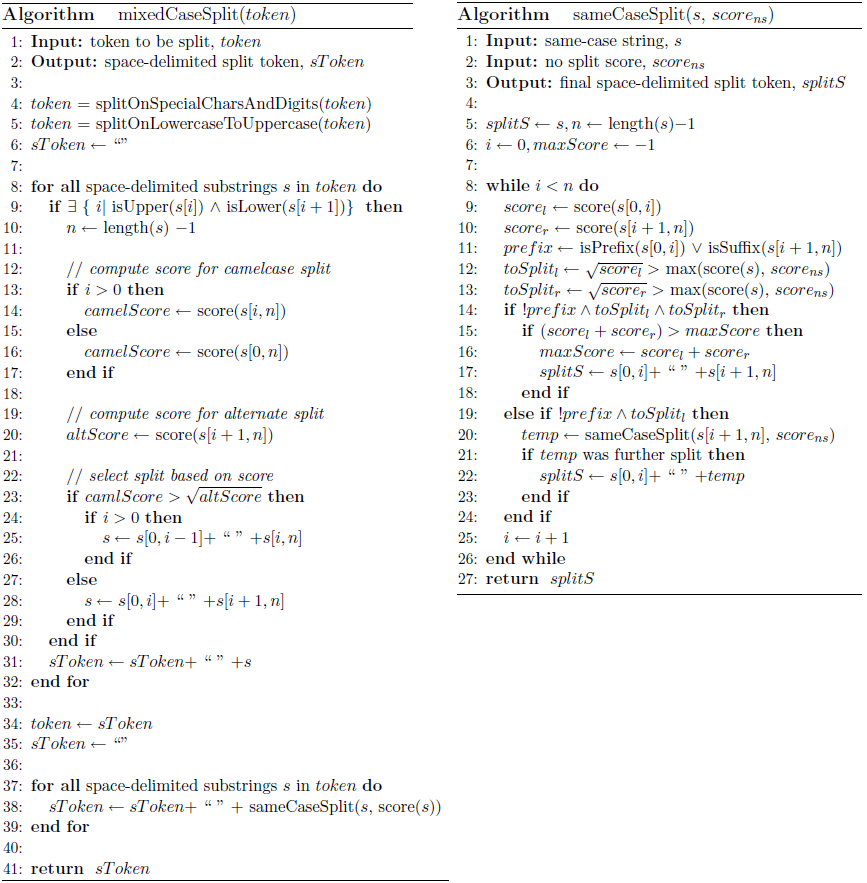
\includegraphics[scale=0.53]{./sam_1.png}
%\caption{Algoritmos mixedCaseSplit y sameCaseSplit}
%\label{sam1}
%\end{figure}

%aclarar que puede recivir distintos tipos de ids ademas de los ya mencionados
El algoritmo ejecuta dos rutinas primero \textit{divisiónHardWord} y después \mbox{\textit{divisiónSoftWord}}. La primera básicamente se encarga de dividir los hardwords (palabras que poseen guión bajo o son del tipo camel-case), luego cada una de las palabras obtenidas son pasadas a la segunda rutina para continuar con el análisis.

En la rutina \textit{divisiónHardWord} (ver algoritmo \ref{AHW}) primero se ejecutan dos funciones (líneas 1 y 2). La primera \textit{dividirCaracteresEspecialesDigitos}, que reemplaza todos los posibles caracteres especiales y números que posea el token por espacio en blanco. La segunda \mbox{\textit{dividirMinusSeguidoMayus}}, de la misma forma que la anterior agrega un blanco entre dos caracteres que sea una minúscula seguido por una mayúscula. En este punto solo quedan tokens de la forma softword o que contengan una mayúscula seguido de minúscula (Ejemplos: \textsf{List, ASTVisitor, GPSstate, state, finalstate, MAX}).

Los casos de softword que se obtuvieron (\textsf{finalstate}, \textsf{MAX}) van directo a la rutina \mbox{\textit{divisiónSoftWord}}.
El resto del tipo mayúscula seguido de minúscula (\textsf{List, ASTVisitor, GPSstate}) continúa con el proceso de división. Aquí se encontrarán casos del tipo \mbox{camel-case} donde la mayúscula indica el comienzo de la nueva palabra (ejemplo: \textsf{List}). Sin embargo, el autor a través de estudios de datos, se encontró con variantes en donde la mayúscula indica el fin de una palabra (ejemplo: \textsf{SQLlist}).
 
El algoritmo decide entre ambas opciones calculando el puntaje (score) de la parte derecha de las dos divisiones (líneas 7 y 8). Aquella con puntaje más alto entre las dos será por la cual se decida (línea 9). Tomando como ejemplo el id \textsf{GPSstate}, para el caso camel-case calculará \textit{score(Sstate)} y para la otra variante \textit{score(state)}. Lógicamente, la función score elegirá \textit{state} sobre \textit{sstate} ya que esta última tiene un puntaje inferior, por ende \textsf{GPSstate} se corresponde a la variante de camel-case. La división elegida se lleva a cabo en las líneas 11 y 13 (según el caso).
Finalmente, todas las partes divididas se envían a \mbox{\textit{divisiónSoftWord} (línea 18)}.
%Para esclarecer más ambas opciones: a) que la separación se realice entre el cambio de mayúscula y minúscula (ejemplo: \textsf{GPS state} - línea 11).

%b) Que se a haga antes de la primer mayúscula siguiendo con la filosofía camel-case (ejemplo: \textsf{GP Sstate} - línea 13). Para este caso, la opción correcta debe ser la a), ya que \textsf{state} debe tener mayor puntaje que \textsf{Sstate}.



\begin{algorithm}
\LinesNumbered%enumera las lineas
\SetKwInOut{Input}{Entrada}\SetKwInOut{Output}{Salida}
\Input{\textbf{\textit{token}} \tcp{\textit{token a dividir}}}
\Output{\textbf{\textit{tokenSep}} \tcp{\textit{token separado con espacios}}}
\BlankLine
\textbf{\textit{token}} $\leftarrow $ dividirCaracteresEspecialesDigitos(\textbf{\textit{token}})

\textbf{\textit{token}} $\leftarrow $ dividirMinusSeguidoMayus(\textbf{\textit{token}})

\textbf{\textit{tokenSep}} $\leftarrow $ “”
\BlankLine
\ForAll{$($Para cada substring \textbf{\textit{s}} separado por ` ' en \textbf{\textit{token}}$)$}{
\BlankLine

\If{$($ $\exists \{ i|esMayus(\textbf{s}[i]) \land esMinus(\textbf{s}[i+1]) \}$ $)$}{
\BlankLine
$n \leftarrow$ length(\textbf{\textit{s}}) $-$ 1
\BlankLine
\tcp{\textit{se determina con la función score si es del tipo camelcase u otra alternativa}} 
\BlankLine
$scoreCamel \leftarrow$ score(\textbf{\textit{s}}[i,n])   

$scoreAlter \leftarrow$ score(\textbf{\textit{s}}[i+1,n])  
\BlankLine
\If{$(scoreCamel > \sqrt{scoreAlter})$}{
\BlankLine
\If{$($i $>$ 0$)$}{
\BlankLine
\textbf{\textit{s}} $\leftarrow$ \textbf{\textit{s}}[0,i $-$ 1] + ` ' + \textbf{\textit{s}}[i,n] \tcp{\textit{GP Sstate}}
}

}\Else{
\BlankLine
\textbf{\textit{s}} $\leftarrow$ \textbf{\textit{s}}[0,i] $+$ ` ' $+$ \textbf{\textit{s}}[i $+$ 1,n]  \tcp{\textit{GPS state}}
}

}
\BlankLine
\textbf{\textit{tokenSep}} $\leftarrow$ \textbf{\textit{tokenSep}} $+$ ` ' $+$\textbf{\textit{s}}

}
\BlankLine
\textbf{\textit{token}} $\leftarrow$ \textbf{\textit{tokenSep}}

\textbf{\textit{tokenSep}} $\leftarrow$ ` '
\BlankLine
\ForAll{$($Para cada substring \textbf{\textit{s}} separado por ` ' en \textbf{token}$)$}{
\BlankLine
\textbf{\textit{tokenSep}} $\leftarrow$ \textbf{\textit{tokenSep}} $+$ ` ' $+$ \textbf{divisiónSoftWord}(\textbf{\textit{s}},score(\textbf{\textit{s}}))
}
\BlankLine
\Return \textbf{\textit{tokenSep}}

\caption{divisiónHardWord \label{AHW}}
\end{algorithm}

La rutina recursiva \textit{divisiónSoftWord} (ver algoritmo \ref{ASW}) recibe como entrada un substring \textbf{\textit{s}}, el cual puede tener tres tipos de variantes: a) todos los caracteres en minúsculas, b) todos con mayúsculas, c) el primer caracter con mayúscula seguido por todas minúsculas (\textsf{Visitor}). El otro parámetro de entrada es el puntaje original \textbf{\textit{score$_{sd}$}} que corresponde a  \textbf{\textit{s}}.

La rutina primero examina cada punto posible de división en \textbf{\textit{s}} dividiendo en \textbf{\textit{split$_{izq}$}} y \textbf{\textit{split$_{der}$}} respectivamente (líneas 4 y 5). La decisión de cual es la mejor división se basa en a) substrings que no tengan prefijos o sufijos conocidos, los mismos están disponibles en la página web del autor\footnote[1]{Listas de prefijos y sufijos  http://www.eecis.udel.edu/˜enslen/Site/Samurai.} (línea 6), b) el puntaje de la división elegida sobresalga del resto de los puntajes (líneas 7-9). 

%una sola division no se llama recursivamente (!prefix ^ toSplitl ^ toSplitr)
Para aclarar el punto anterior, para cada partición (izquierda o derecha) obtenida se calcula el score (líneas 4 y 5). Luego este es comparado con el puntaje de la palabra original (\textbf{\textit{score$_{sd}$}} score original) y el puntaje de la palabra actual (score(\textbf{\textit{s}})) . En un principio ambas son iguales pero a medida que avanza la recursión score(\textbf{\textit{s}}) varia con respecto a \textbf{\textit{score$_{sd}$}} (líneas 7 y 8).
%agregar ejemplos gráficos etc.

%si se cumple solo la parte izquierda se llama recursivamente (!prefix ^ toSplitl)
En caso de que no tenga prefijos y sufijos ordinarios, se considera que la parte izquierda es un candidato. Por otro lado, la cadena de la parte derecha se invoca recursivamente con la rutina porque podría seguir dividiéndose en más partes (línea 14).

Si la parte derecha finalmente se divide, luego entre la parte izquierda y la derecha también. Por ejemplo el id \textsf{countrownumber} primero se analiza \textsf{rownumber}(parte derecha - línea 14) como este finalmente se separará en \mbox{\textsf{row number}}, la palabra \textsf{count} (parte izquierda) se divide del resto (línea 16) dando como resultado \textsf{count row number}. Sin embargo, cuando la parte derecha no es dividida tampoco se debería separar entre ambas partes (el \textsf{if} de la línea 13 controla esto). Los análisis de datos hechos por el autor \cite{EHPV09} obligan a hacer este control ya que se encontraron abundantes casos erróneos de división, uno de ellos es \textsf{string ified}. 


%que no se debe separar la actual posición, en base solo a la evidencia en la izquierda ya que puede ser erróneo, un caso conocido erróneo es \textsf{string ified}. 

%La ejecución recursiva de samurai para la cadena \textsf{nonnegativedecimaltype} se ejecuta correctamente y da como resultado \textsf{nonnegative decimal type} \cite{EHPV09}.

Otro problema detectado son las palabras de pocos caracteres (menor a 3). Estas palabras, tienen mucha aparición en los códigos y por lo general el puntaje es más alto que el resto. Por esta razón, el autor \cite{EHPV09} en base a un análisis sustancial decide colocar la raíz cuadrada en algunos resultados de score antes de comparar (línea 7 y 8), sino la división frecuentemente seria errónea. Un ejemplo es la palabra \mbox{\textsf{per formed}}. La presencia de la raíz cuadrada en el algoritmo \textit{divisiónHardWord} (línea 9), cuando se compara el caso camel-case y el caso alternativo también es para solucionar este problema.\\

\begin{algorithm}
\LinesNumbered%enumera las lineas
\SetKwInOut{Input}{Entrada}\SetKwInOut{Output}{Salida}
\Input{\textbf{\textit{s}} \tcp{\textit{softword string}}}
\Input{\textbf{\textit{score$_{sd}$}} \tcp{\textit{puntaje de s sin dividir}}}
\Output{\textbf{\textit{tokenSep}} \tcp{\textit{token separado con espacios}}}
\BlankLine%espacio en blanco

\textbf{\textit{tokenSep}} $\leftarrow$ \textbf{\textit{s}}, n $\leftarrow$ length(\textbf{\textit{s}}) - 1

i $\leftarrow$ 0, \textbf{\textit{maxScore}} $\leftarrow -$ 1
\BlankLine

\While{$($i $<$ n$)$}{
\BlankLine
\textbf{\textit{score$_{izq}$}} $\leftarrow$ score(\textbf{\textit{s}}[0,i])

\textbf{\textit{score$_{der}$}} $\leftarrow$ score(\textbf{\textit{s}}[i+1,n])
\BlankLine
\textbf{\textit{preSuf}} $\leftarrow$ esPrefijo(\textbf{\textit{s}}[0,i]) $\vee$ esSufijo(\textbf{\textit{s}}[i+1,n])
\BlankLine
\textbf{\textit{split$_{izq}$}} $\leftarrow$  $\sqrt{score_{izq}} >$ max(score(\textbf{\textit{s}}),\textbf{\textit{score$_{sd}$}})

\textbf{\textit{split$_{der}$}} $\leftarrow$  $\sqrt{score_{der}} >$ max(score(\textbf{\textit{s}}),\textbf{\textit{score$_{sd}$}})
\BlankLine

\If{$($!\textbf{\textit{presuf}} $\land$ \textbf{\textit{split$_{izq}$}} $\land$ \textbf{\textit{split$_{der}$}}$)$}{
\BlankLine
\If{$(($\textbf{\textit{split$_{izq}$}} $+$ \textbf{\textit{split$_{der}$}}$)$ $>$ \textbf{maxScore}$)$}{
\BlankLine
\textbf{\textit{maxScore}} $\leftarrow$ (\textbf{\textit{split$_{izq}$}}$+$\textbf{\textit{split$_{der}$}})

\textbf{\textit{tokenSep}} $\leftarrow$ \textbf{\textit{s}}[0,i] + ` ' + \textbf{\textit{s}}[i+1,n]
}

}\ElseIf{$(!$\textbf{\textit{presuf}} $\land$ \textbf{\textit{split$_{izq}$}}$)$}{
\BlankLine
\textbf{\textit{temp}} $\leftarrow$ \textbf{divisiónSoftWord}(\textbf{\textit{s}}[i+1,n],\textbf{\textit{score$_{sd}$}})

\If{$($\textbf{\textit{temp}} se dividió?$)$}{
\textbf{\textit{tokenSep}} $\leftarrow$ \textbf{\textit{s}}[0,i] + ` ' + \textbf{\textit{temp}}
}

}
\BlankLine
i $\leftarrow$ i+1
}
\BlankLine
\Return \textbf{\textit{tokenSep}}

\caption{divisiónSoftWord \label{ASW}}
\end{algorithm}

\pagebreak
\noindent \textbf{Función de Scoring}

Para que la técnica samurai pueda llevar a cabo la tarea de separación de ids, se necesita la función de scoring. Como bien se explicó anteriormente esta función participa en 2 decisiones claves durante el proceso de división:

\begin{itemize}
\itemsep0em%reduce espacio
\item En la rutina \textit{divisiónHardWord}, para determinar si el la división del id es un caso de camel-case o no (líneas 7 y 8).

\item En la rutina \textit{divisiónSoftWord}, para puntuar las diferentes particiones de substrings y elegir la mejor separación (líneas 4, 5, 7 y 8).
\end{itemize}

Dado un string \textbf{s}, la función \textit{score(\textbf{s})} indica i) la frecuencia de aparición de \textbf{s} en el programa bajo análisis y ii) la frecuencia en un conjunto grande de programas predefinidos. La fórmula es la siguiente:

\begin{center}
$Frec(s,p) + ( globalFrec(s) / \log_{10}(totalFrec(p) )$
\end{center}

Donde \textbf{p} es el programa de estudio, $Frec(s,p)$ es la frecuencia de ocurrencia de \textbf{s} en \textbf{p}. La función $totalFrec(p)$, es la frecuencia total de todos los strings en el programa \textbf{p}. La función $globalFrec(s)$, es la frecuencia de aparición de \textbf{s} en una gran conjunto de programas tomados como muestras\footnote[1]{Estos programas son alrededor de 9000 y están escritos en JAVA} \cite{EHPV09}.

\pagebreak
\subsection{Algoritmo de Expansión Básico}
%noindent elimina sangria
%\noindent \textbf{Algoritmo 1}

El algoritmo de expansión de abreviaturas ideado por Lawrie, Feild, Binkley (mismos autores que la técnica de separación Greedy) \cite{LFBEX07} trabaja con cuatro listas para realizar su tarea:

\begin{itemize}
\itemsep0em%reduce espacio
\item Una lista de palabras (en lenguaje natural) que se extraen del código.
\item Una lista de frases (en lenguaje natural) presentes también en el código.
\item Una lista de palabras irrelevantes (stop list).
\item Una lista de palabras de un diccionario en inglés.
\end{itemize}

La primer lista se confecciona de la siguiente manera, para cada método \textit{f} dentro del código se crea una lista de palabras que se extraen de los comentarios que están antes (comentarios JAVA Doc) o dentro del método \textit{f}. También se incorporan los ids del tipo hardword (si existen) dentro del alcance local de \textit{f}. 

La lista de frases se arma utilizando una técnica que extrae frases en lenguaje natural \cite{FFCW01}, el principal recurso son los comentarios y los ids multi-palabras. En este punto se construye un acrónimo\footnote[1]{Abreviación formada por las primeras letras de cada palabra en una frase. Ejemplo gif: Graphics Interchange Format.} con las palabras de alguna frase, si ese acrónimo coincide con alguno de los ids extraídos, entonces esa frase se considera como potencial expansión (Ejemplo: la frase \textsf{file status} es una expansión posible para el id \textsf{fs\_exists} $\rightarrow$ \textsf{file status exists}).

Una vez que las listas de palabras y frases potenciales se confeccionan, la ejecución del algoritmo comienza. Este algoritmo (ver algoritmo \ref{BEA}) recibe como entrada la abreviatura a expandir y las 4 listas antes descriptas. El primer paso es ver si la abreviatura forma parte de la lista de palabras irrelevantes (stop-list línea 1)\footnote[2]{Esta lista se usa con la misma política que el algoritmo Greedy.}. En caso de que así sea, no se retornan resultados. La razón de esto es porque estas palabras no aportan información importante en la comprensión del código y son fácilmente reconocidas por los ingenieros del software. Algunos casos son artículos/conectores (the, an, or) y palabras reservadas del lenguaje de programación que se utilicen (\textsf{while, for, if,} etc.).

\begin{algorithm}
\LinesNumbered%enumera las lineas
\SetKwInOut{Input}{Entrada}\SetKwInOut{Output}{Salida}
\Input{\textit{\textbf{abrev}} \tcp{\textit{Abreviatura a expandir}}}
\Input{\textit{\textbf{wordList}} \tcp{\textit{Palabras extraídas del código}}}
\Input{\textit{\textbf{phraseList}} \tcp{\textit{Frases extraídas del código}}}
\Input{\textit{\textbf{stopList}} \tcp{\textit{Palabras Excluyentes}}}
\Input{\textit{\textbf{dicc}} \tcp{\textit{\textit{Diccionario en Inglés}}}}
\Output{\textbf{únicaExpansión} \tcp{\textit{Abreviatura expandida, o null}}}
\BlankLine

\If{$($\textit{\textbf{abrev}} $\in$ \textit{\textbf{stopList}}$)$}{
\Return null
}
\BlankLine
listaExpansión $\leftarrow$ [ ]
\BlankLine
\tcp{\textit{Buscar coincidencia de acrónimo.}}

\ForAll{$($Para cada frase \textit{\textbf{phrase}} en \textit{\textbf{phraseList}}$)$}{
\BlankLine

\If{$($ $\exists \{$\textbf{phrase} $|$ \textit{\textbf{abrev}} es un acrónimo de \textit{\textbf{phrase}}$\}$ $)$}{
listaExpansión.add(\textit{\textbf{phrase}}) 
}
}

\BlankLine
\tcp{\textit{Buscar abreviatura común.}}

\ForAll{$($ Para cada palabra \textit{\textbf{word}} en  \textit{\textbf{wordList}} $)$}{
\BlankLine
\If{ $($ $\exists \{$\textbf{word} $|$ \textit{\textbf{abrev}} es una abreviatura de \textit{\textbf{word}}$\})$}{
listaExpansión.add(\textit{\textbf{word}}) 
}

}

\BlankLine
\tcp{\textit{Si no hay éxito, buscar en el diccionario.}}

\If{$($isEmpty$($listaExpansión$))$}{
\BlankLine
listaCandidatos $\leftarrow$ buscarDiccionario(\textit{\textbf{abrev}},\textit{\textbf{dicc}})
listaExpansión.add(listaCandidatos)
}


\BlankLine
\textbf{únicaExpansión} $\leftarrow$ null
\BlankLine
\tcp{\textit{Debe haber un solo resultado, sino no retorna nada.}}

\If{$($length$($listaExpansión$)$ $=$ 1$)$}{
\BlankLine
\textbf{únicaExpansión} $\leftarrow$ listaExpansión[0]
}
\BlankLine
\Return \textbf{únicaExpansión} 

\caption{Expansión Básica \label{BEA}}
\end{algorithm}

Siguiendo con la ejecución, se chequean si alguna de las frases extraídas del código se correspondan con la abreviatura en forma de acrónimo (línea 5). %Esto ocurre cuando las primeras letras de cada palabra en la frase se corresponde con las letras de la abreviatura en el mismo orden.

Después, se busca si las letras de la abreviatura coinciden en el mismo orden que las letras de una palabra presente en la lista de palabras recolectadas del código (línea 8). Ejemplos: \textsf{horiz} $\rightarrow$ \textsf{horizontal}, \textsf{trgn} $\rightarrow$ \textsf{triangle}.

En caso de no tener éxito, la búsqueda continúa en el diccionario predefinido como último recurso (línea 11).

%al igual que samurai stop list y steming usa tecnicas de ir - completar si es necesario

Esta técnica de expansión descripta, solo retorna una única expansión potencial para una abreviatura determinada y en caso contrario no retorna nada (líneas 13 y 14). El motivo de esto, es porque no tiene programado como decidir una sola opción ante múltiples alternativas de expansión. A esta característica, los autores lo presentan como trabajo futuro \cite{LFBEX07,EZH08}.

\subsection{Algoritmo de Expansión AMAP}
%noindent elimina sangria
%\noindent \textbf{\\Algoritmo 2}

El algoritmo de expansión de abreviaturas que construyó Emily Hill, Zachary Fry, Haley Boyd \cite{EZH08} conocido como \textit{Automatically Mining Abbreviation Expansions in Programs} (AMAP), además de buscar expansiones potenciales al igual que el algoritmo anterior, también se encarga de seleccionar la que mejor se ajusta en caso de que haya más de un resultado posible. Otra mejora destacable, con respecto al algoritmo previo es que no se necesita un diccionario con palabras en lenguaje natural. Los diccionarios (en inglés) incluyen demasiadas palabras e implica disponer de un gran almacenamiento. 

Las fuentes de palabras que se utilizan son una lista de abreviaciones comunes. Estas abreviaciones se obtienen automáticamente desde distintos programas. También se puede incorporar palabras en forma personalizada. La lista palabras irrelevantes (stop-list) y la de contracciones más comunes se arman manualmente.

Para agilizar la lectura se asigna el nombre de “palabras largas” a las palabras normales que no están abreviadas y son potenciales expansiones de las abreviadas.

La técnica automatizada AMAP busca palabras largas candidatas para una palabra abreviada dentro del código con la misma filosofía que se usa en la construcción de una tabla de símbolos en un compilador.

Se comienza con el alcance estático más cercano donde se examinan sentencias vecinas a la palabra abreviada. Luego gradualmente el alcance estático crece para incluir métodos, comentarios de métodos, y los comentarios de la clase. Si la técnica no encuentra una palabra larga adecuada para una determinada palabra abreviada, la búsqueda continúa mirando todo el programa y finalmente examina las librerías de JAVA SE 1.5. 

Los autores asumen que una palabra abreviada está asociada a una sola palabra larga dentro de un método. No es frecuente que dentro de un método una palabra abreviada posea más de una expansión posible. En caso de que esto se cumpla, se puede cambiar la asunción. Se puede estipular que una palabra abreviada solo tiene una sola expansión posible dentro de los bloques o achicando aun más solo dentro de las sentencias de código.

%A continuación, se explica los pasos que ejecuta la herramienta AMAP: 
%\begin{enumerate}
%\itemsep0em%reduce espacio
%\item Como se realiza la búsqueda para encontrar palabras largas candidatas dentro de un método. 
%\item Como se elije entre múltiples alternativas cual es la mejor expansión.
%\item Como se buscan nuevas palabras si el alcance local del método no es suficiente, a través del método EMF (Expansión más Frecuente). 
%\end{enumerate}

El algoritmo AMAP ejecuta los siguientes pasos:

\begin{enumerate}
\itemsep0em%reduce espacio
\item Buscar palabras largas canditas dentro de un método.
\item Elegir la mejor alternativa de expansión.
\item Buscar nuevas palabras si en el alcance local no es suficiente utilizando el método EMF (Expansión más Frecuente).
\end{enumerate}

A continuación se explican cada uno de esos métodos.\\

Comenzando por el ítem 1, la búsqueda de las palabras largas contiene dos algoritmos, uno que recibe como entrada palabras abreviadas compuestas por una sola palabra (singulares) y el otro algoritmo se encarga de procesar multi-palabras.\\

\noindent \textbf{Búsqueda por Palabras Singulares\\}

El primer paso para buscar palabras largas consiste en construir una expresión regular con un patrón de búsqueda.  Este patrón se encarga de seleccionar las palabras largas que coincidan con las letras de la palabra abreviada.

Los patrones se construyen a partir de la palabra abreviada, a continuación se detalla como se arman estos patrones: 

\begin{description}
\itemsep0em%reduce espacio
\item[Patrón prefijo:] Se construye colocando la palabra abreviada (\textit{\textbf{pa}}) seguida da la expresión regular [a-z]+. Las palabras que coinciden si o si deberán comenzar con \textit{\textbf{pa}}. La expresión regular queda: \textit{\textbf{pa}}[a-z]+.

Ejemplo: El patrón \textsf{arg}[a-z]+ coincide (entre otras) con la palabra \textit{\textbf{arg}}ument.

\item[Patrón compuesto por letras:]  La expresión regular se construye insertando [a-z]* después de cada letra de la palabra abreviada (\textit{\textbf{pa}}). Si \textit{\textbf{pa}}$=c_{1},c_{2},c_{3},..,c_{n}$, donde $n$ es la longitud de la palabra abreviada. El patrón queda: $c_{1}$[a-z]*$c_{2}$[a-z]*$c_{3}$[a-z]*..$c_{n}$.

Ejemplo: El patrón \textsf{p}[a-z]*\textsf{g}[a-z]*\textsf{m}[a-z]* coincide (entre otras) con  \textit{\textbf{p}}ro\textit{\textbf{g}}ra\textit{\textbf{m}}.
\end{description}


%\begin{figure}[h] %[h] para here [b] para bottom [t] para top
%\centering
%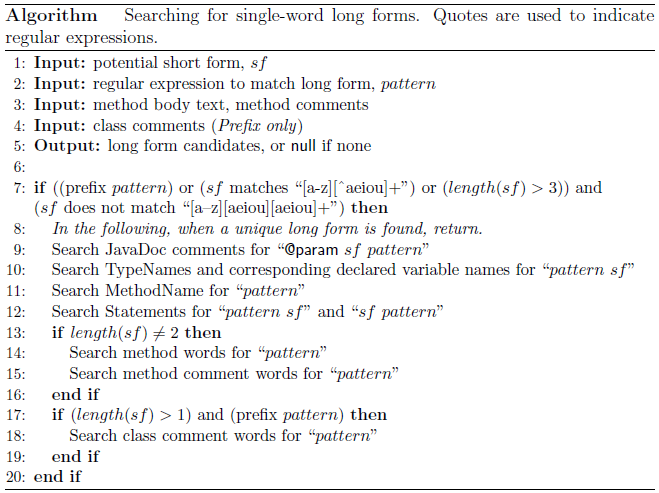
\includegraphics[scale=0.7]{./exp_1.png}
%\caption{Algoritmo de Expansión de una sola Palabra.}
%\label{exp1}
%\end{figure}

La búsqueda de palabras singulares se presenta en el algoritmo \ref{BPS}. Los parámetros de entrada son la palabra abreviada a expandir, la expresión regular formada por el patrón elegido, los distintos comentarios que existan en el código (en la clase y en el método) y el cuerpo del método.

En la línea 1 se impide básicamente dos cosas: 

a) Que no se procesen palabras abreviadas con muchas vocales consecutivas (segundo argumento del \textsf{and} en el \textsf{if}). La autora de AMAP comprobó \cite{EZH08} que la mayoría de las palabras abreviadas con vocales consecutivas se expanden como multi-palabras (ejemplos: es el caso de los acrónimos \textsf{gui} $\rightarrow$ \textsf{graphical user interface}, \textsf{ioe} $\rightarrow$ \textsf{invalid object exception}). El algoritmo de la próxima sección es el encargado de expandirlos.

b) En caso de que el patrón sea el \textit{compuesto por letras} (no sea el prefijo), se hacen dos controles más (primer argumento del \textsf{and} en el \textsf{if}). Uno es, que la abreviatura no posea muchas vocales consecutivas (“[\^{}aeiou]+” logra eso) y la otra es que longitud sea mayor a 3. La autora a través del análisis de datos determino esta restricción \cite{EZH08}, ya que el \textit{patrón compuesto por letras} tiene el inconveniente que es muy flexible y tiende a capturar muchas palabras largas incorrectas. Por ejemplo: \textsf{lang} $\rightarrow$ \textsf{loading}, \textsf{language} o también \textsf{br} $\rightarrow$ \textsf{bar}, \textsf{barrier}, \textsf{brown}.

En las líneas 2-10 se describe el proceso de búsqueda. Si alguna de estas sentencias de búsqueda encuentran un sola palabra larga candidata, el algoritmo finaliza y retorna el resultado. 

\begin{algorithm}
\LinesNumbered%enumera las lineas
\SetKwInOut{Input}{Entrada}\SetKwInOut{Output}{Salida}
\Input{\textit{\textbf{pa}} \tcp{\textit{Palabra Abreviada}}}
\Input{\textit{\textbf{patrón}} \tcp{\textit{Expresión regular}}}
\Input{Cuerpo y Comentarios del Método}
\Input{Comentarios de la Clase}
\Output{Palabras largas candidatas, o null si no hay}
\BlankLine
\tcp{\textit{Las expresiones regulares están entre comillas}}
\BlankLine

\If{ $($\textbf{patrón} prefijo $\vee$ \textit{\textbf{pa}} coincide “[a-z][aeiou]$+$” $\vee$ length(\textit{\textbf{pa}}) $>$ 3$)$ $\land$ $($\textit{\textbf{pa}} no coincide con “[a-z][aeiou][aeiou]$+$”$)$}{


\BlankLine
\tcp{\textit{Si alguna de las siguientes búsquedas encuentra un único resultado, el algoritmo lo retorna finalizando la ejecución}}
\BlankLine
Buscar en Comentarios JavaDoc con “\textsf{\at param} \textit{\textbf{pa patrón}}”
\BlankLine
Buscar en Nombres de Tipos y la correspondiente Variable declarada con “\textit{\textbf{patrón pa}}”
\BlankLine
Buscar en el Nombre del Método con “\textit{\textbf{patrón}}”
\BlankLine
Buscar en las Sentencias con “\textit{\textbf{patrón pa}}” y “\textit{\textbf{pa patrón}}”
\BlankLine
\If{$($length(\textit{\textbf{pa}} $\neq$ 2)$)$}{
\BlankLine
Buscar en palabras del Método con “\textit{\textbf{patrón}}”
\BlankLine
Buscar en palabras que están en los Comentarios del Método con “\textit{\textbf{patrón}}”

}

\If{$($length(\textit{\textbf{pa}} $>$ 1)$)$ $\land$ $($\textit{\textbf{patrón}} prefijo$)$}{
\BlankLine
\tcp{\textit{Solo se busca con patrones prefijos}}

Buscar en palabras que están en los Comentarios de la Clase con “\textit{\textbf{patrón}}”
}
}

\caption{Búsqueda por Palabras Singulares \label{BPS}}
\end{algorithm}

En la línea 2 la búsqueda se realiza en los comentarios Java Doc, donde la expresión regular es “\at param \textit{\textbf{pa}} \textit{\textbf{patrón}}”. Por ejemplo, si en Java Doc se tiene el comentario “\at param ind index” donde \textit{\textbf{pa}} = \textbf{ind}, \textit{\textbf{patrón}} = \mbox{“ind[a-z]+”}. La expresión regular \mbox{“\at param ind ind[a-z]+”} coincidirá y devolverá el resultado  “index” como expansión de \textbf{ind}.

Si no hay resultados, sigue la búsqueda en la línea 3 con los nombres de los tipos ubicados en las variables declaradas, donde la expresión regular es “\textit{\textbf{patrón}} \textit{\textbf{pa}}”. Por ejemplo si se tiene una declaración “\textbf{component comp}” donde \textit{\textbf{pa}} = \textbf{comp}, \textit{\textbf{patrón}} = “comp[a-z]+”  la expresión regular \mbox{“comp[a-z]+ comp”} coincidirá y devolverá el resultado  “component” como expansión de \textbf{comp}.

Si no tiene éxito sigue en la línea 4 donde se busca coincidir con “\textit{\textbf{patrón}}” en el nombre del método. En caso de seguir sin resultado alguno, prosigue en la línea 5 con distintas variantes “\textit{\textbf{patrón}} \textit{\textbf{pa}}” o “\textit{\textbf{pa}} \textit{\textbf{patrón}}” en las sentencias comunes del método. 

%En la figura \ref{exp3} se pueden observar los distintos casos que se describieron.

Si la ejecución continúa, la línea 6 se restringe una búsqueda por palabras que tengan al menos 3 caracteres ya que generalmente aquellas con 2 tienden a ser multi-palabras (Ejemplo: \textsf{fl $\rightarrow$ file system} / ver próxima sección). Luego en la línea 7 se busca con \textit{\textbf{patrón}} solamente en palabras del método (ejemplo: para una abreviatura \textsf{setHor} coincide con una función \textsf{setHorizontal()}). Después en la línea 8 se busca en palabras de comentarios dentro del método con \textit{\textbf{patrón}}.

Para finalizar, en la línea 10 si la palabra abreviada tiene más de un caracter y el patrón es de tipo prefijo, se busca usando (\textit{\textbf{patrón}}) en los comentarios de la clase. En la línea 9 se restringe esta búsqueda, porque la autora sostiene \cite{EZH08}, que buscar con un solo caracter en comentarios implica tener muchos resultados y más aun si el patrón es el compuesto por letras.\\

%\pagebreak
\noindent \textbf{Búsqueda por Multi-Palabras\\}

El algoritmo de búsqueda por multi-palabras a diferencia del explicado anteriormente, expande abreviaturas que contienen dos o más palabras. Algunos ejemplos son: \textsf{gui $\rightarrow$ graphical user interface, fl $\rightarrow$ file system}. Como bien se definió en secciones anteriores estas abreviaturas se las conoce con el nombre de acrónimos, que generalmente están conformadas por 2 ó 3 caracteres. El algoritmo anterior intenta detectar este tipo de abreviaturas y no analizarlas para que sea procesado por el multi-palabras.

Al igual que el algoritmo de palabras singulares, el algoritmo de multi-palabras utiliza expresiones regulares conformada por patrones de búsqueda. Los patrones utilizados en las búsquedas multi-palabras se construyen de la siguiente manera:

%Al igual que la búsqueda por palabras singulares, la búsqueda por multi-palabras se va incrementando en el alcance de código hasta encontrar un candidato que coincida con el patrón. Sin embargo, es importante tener en cuenta hasta donde los patrones multi-palabras realizan la búsqueda. Por ejemplo, una abreviatura \textsf{il} puede coincidir con la frase “\textbf{i}t is importante to \textbf{l}imit” en la sentencia anterior donde se encuentra \textsf{il}. Por eso, se preprocesa el texto y los comentarios dentro del método sin ir mas allá de las declaraciones y de los ids propios del método.

%También se dividen los comentarios y los literales strings en frases usando signos de puntuación (?!,;).

%Las abreviaciones como \textsf{val} no se expanden a \textsf{verify and load}, por que las palabras irrelevantes (stop words) se remueven de los comentarios (en este caso \textsf{and}) en el cuerpo del método.



\begin{description}
\itemsep0em%reduce espacio
\item[Patrón acrónimo:] Se elabora colocando la expresión regular [a-z]+[ ]+, después de cada letra de la palabra abreviada (\textit{\textbf{pa}}). Si \textit{\textbf{pa}}$=c_{1},c_{2},c_{3},..,c_{n}$, donde $n$ es la longitud de la palabra abreviada. El patrón queda: \mbox{$c_{1}$[a-z]+[ ]+$c_{2}$[a-z]+[ ]+$c_{3}$[a-z]+[ ]+..[a-z]+[ ]+$c_{n}$}. Permite encontrar acrónimos tales como \textsf{xml} $\rightarrow$ e\textbf{\textit{x}}tensible \textbf{\textit{m}}arkup \textbf{\textit{l}}anguage.

\item[Patrón de Combinación de Palabras:] En este caso el patrón se construye de manera similar al anterior pero se usa la expresión regular [a-z]*?[ ]*? después de cada caracter de la palabra abreviada (\textit{\textbf{pa}}). Si \textit{\textbf{pa}}$=c_{1},c_{2},c_{3},..,c_{n}$, donde $n$ es la longitud de la palabra abreviada. El patrón queda: $c_{1}$[a-z]*?[ ]*?$c_{2}$[a-z]*?[ ]*?$c_{3}$[a-z]*?[ ]*?...[a-z]*?[ ]*?$c_{n}$. De esta manera se pueden capturar palabras del tipo \textsf{arg} $\rightarrow$ \textbf{\textit{a}}ccess \textbf{\textit{r}}i\textbf{\textit{g}}hts, permitiendo más capturas que el patrón anterior.
\end{description}


%\begin{figure}[h] %[h] para here [b] para bottom [t] para top
%\centering
%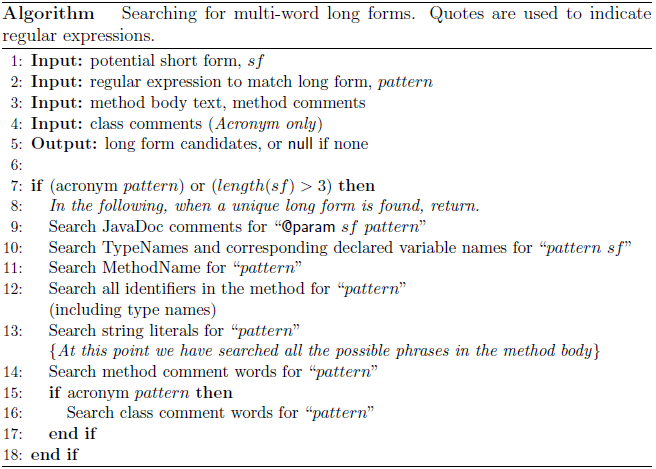
\includegraphics[scale=0.7]{./exp_2.png}
%\caption{Algoritmo de Expansión Multi-Palabra.}
%\label{exp2}
%\end{figure}

En el algoritmo \ref{BMP}, se presenta la búsqueda por multi-palabras \cite{EZH08}. Las variables de entrada son: la abreviatura multi-palabra a expandir, la expresión regular formada por el patrón elegido, los distintos comentarios que existan en el código (en la clase y en el método) y el cuerpo del método.

\begin{algorithm}
\LinesNumbered%enumera las lineas
\SetKwInOut{Input}{Entrada}\SetKwInOut{Output}{Salida}
\Input{\textit{\textbf{pa}} \tcp{\textit{Palabra Abreviada}}}
\Input{\textit{\textbf{patrón}} \tcp{\textit{Expresión regular}}}
\Input{Cuerpo y Comentarios del Método}
\Input{Comentarios de la Clase}
\Output{Palabras largas candidatas, o null si no hay}
\BlankLine
\tcp{\textit{Las expresiones regulares están entre comillas}}
\BlankLine

\If{$($\textit{\textbf{patrón}} acrónimo $\vee$ length(\textit{\textbf{pa}}) $>$ 3$)$}{

\BlankLine
\tcp{\textit{Si alguna de las siguientes búsquedas encuentra un único resultado, el algoritmo lo retorna finalizando la ejecución}}
\BlankLine
Buscar en Comentarios JavaDoc con “\textsf{\at param} \textit{\textbf{pa patrón}}”
\BlankLine
Buscar en Nombres de Tipos y la correspondiente Variable declarada con “\textit{\textbf{patrón pa}}”
\BlankLine
Buscar en el Nombre del Método con “\textit{\textbf{patrón}}”
\BlankLine
Buscar en todos los ids (y sus tipos) dentro del Método con “\textit{\textbf{patrón}}”
\BlankLine
Buscar en Literales String con “\textit{\textbf{patrón}}”
\BlankLine
\tcp{\textit{En este punto se buscó en todos los lugares posibles dentro del método}}
\BlankLine
Buscar en palabras que están en los Comentarios del Método con “\textit{\textbf{patrón}}”
\BlankLine
\If{$($\textit{\textbf{patrón}} acrónimo$)$}{
\BlankLine
\tcp{\textit{Solo se busca con patrones Acrónimos}}
Buscar en palabras que están en los Comentarios de la Clase con “\textit{\textbf{patrón}}”
}
}

\caption{Búsqueda por Multi Palabras \label{BMP}}
\end{algorithm}

Los patrones de \textit{combinación de palabras} son menos restrictivos que los patrones de \textit{acrónimos} y frecuentemente conllevan a malas expansiones. En caso que no sea acrónimo, la búsqueda se restringe a palabras abreviadas ingresadas con longitud 4 ó mayor (línea 1). Esto genera la sensación de que se pierden casos de 2 ó 3 caracteres pero estudios indican que son la minoría \cite{EZH08}.
 
Al igual que el algoritmo anterior en las líneas 2-4 se realiza la búsqueda primero en comentarios JAVA Doc, luego en nombres de tipos, después en el nombre del método. La Figura \ref{exp3} muestra algunos ejemplos antedichos.

Dado que las expresiones regulares son más complejas en este algoritmo, los tiempos de respuestas tienen cotas más altas. Es por esto que la búsqueda en sentencias no se realiza, a diferencia del algoritmo de palabras singulares.

\begin{figure}[t] %[h] para here [b] para bottom [t] para top
\centerline{%queda centrada mejor la imagen
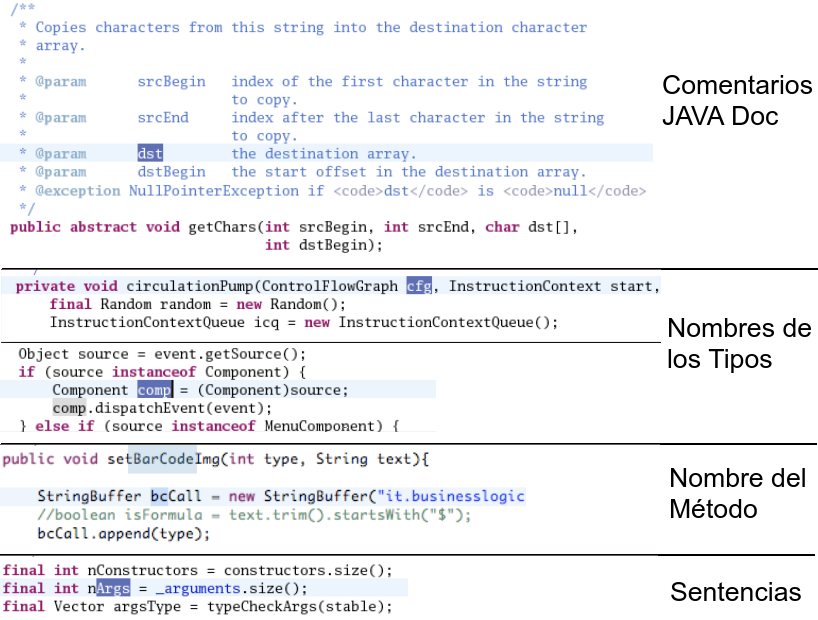
\includegraphics[scale=0.7]{./exp_3.png}
}
\caption{Ejemplos de trozos de Código.}
\label{exp3}
\end{figure}

En las siguientes líneas 5-7 se examinan los ids (incluyendo declaraciones), palabras de literales strings y palabras de comentarios del método. En los tres casos solo se utiliza “\textit{\textbf{patrón}}”.

Luego en la línea 9 se busca en comentarios de la clase con el \textit{patrón acrónimo}. Cabe aclarar que \textit{patrón de combinación de palabras} en este caso no se usa (línea 8) ya que puede tomar palabras largas incorrectas.

Finalmente después de observar cientos de casos de palabras largas, la autora \cite{EZH08} concluye que el mejor orden de ejecución de las técnicas de búsqueda es ejecutar los patrones: acrónimo (multi-palabra), prefijo (una sola palabra), compuesto por letras (una sola palabra), combinación de palabras (multi-palabra).

Si ninguna de las estrategias de expansión funciona en el ámbito local dentro de un método, se procede a buscar la palabra abreviada en un listado de contracciones (inglés).

En caso de seguir sin éxito, se recurre a la técnica conocida como expansión más frecuente (EMF). 

Antes de explicar EMF, esta pendiente describir la forma en que AMAP decide ante varias alternativas de expansión.

\noindent \textbf{\\Decidir entre Múltiples Alternativas\\}

Existe la posibilidad de que una abreviación posea múltiples alternativas potenciales de expansión dentro del mismo alcance estático. Por ejemplo, el patrón prefijo para \textsf{val} puede coincidir \textsf{value} o \textsf{valid}. La técnica de elección entre múltiples candidatos procede de la siguiente manera:

\begin{enumerate}
\itemsep0em%reduce espacio
\item Se elije la palabra larga dentro del alcance estático con mayor frecuencia de aparición. Tomando el ejemplo anterior para \textsf{val} si \textsf{value} aparece 3 veces y \textsf{valid} una sola vez, se elije la primera.

\item En caso de haber paridad en el item 1, se agrupa las palabras largas con similares características. Por ejemplo, si \textsf{def} coincide con \textsf{defaults}, \textsf{default} y \textsf{define} donde todas aparecen 2 veces, en este caso se agrupa las 2 primeras en solo \textsf{default} con una cantidad de 4 predominando sobre \textsf{define}.

\item En caso de que la igualdad persista, se acumulan las frecuencias de aparición entre las distintas búsquedas para determinar un solo candidato. Por ejemplo, si el id \textsf{fs} coincide con \textsf{file system} y \textsf{file socket} ambas con una sola aparición en los comentarios de JAVA Doc. Para llegar a una decisión, primero se almacena ambas opciones. Después, se continua con el resto de las búsquedas (nombres de tipos de ids, literales, comentarios) en cuanto aparezca una de las dos, por ejemplo \textsf{file socket} este termina prevaleciendo sobre \textsf{file system}.

\item Finalmente si todas las anteriores fallan se recurre al método de expansión más frecuente (EMF). 

\end{enumerate}


\noindent \textbf{Expansión Más Frecuente (EMF)\\}


La estrategia EMF \cite{EZH08} es una técnica que se utiliza en 2 casos. Por un lado, 
encuentra una expansión cuando todas las búsquedas fracasan y por el otro, ayuda a decidir entre varias alternativas de expansión. 

La idea consiste en ejecutar la misma estrategia local de expansión de abreviaturas explicada anteriormente pero sobre el programa entero. Para cada palabra abreviada, se cuenta el número de veces que esa palabra se le asigna una palabra larga candidata. Luego se calcula la frecuencia relativa de una palabra abreviada con respecto a cada palabra larga encontrada. La palabra larga con mayor frecuencia relativa se considera la expansión más frecuente. Al final del proceso se agrupan las palabras largas potenciales en un listado de EMF.

Sin embargo, suele pasar que la expansión más probable es la incorrecta. Para evitar que suceda, una palabra larga debe a su vez, superar la frecuencia relativa más de la mitad (0.5). Inclusive, la palabra abreviada debe tener al menos 3 asignaciones de palabras largas candidatas en todo el programa.

La técnica EMF tiene 2 niveles, el primero es a nivel de programa y el otro más general a nivel JAVA. El nivel de programa es ideal ya que expande las abreviaturas con palabras propias del dominio del problema. El nivel más general se arma con la API\footnote[1]{Application Programming Interface} de JAVA. En la tabla \ref{tab_emf} se muestra algunos casos de frecuencias relativas más altas de JAVA 5. En caso de que una palabra abreviada no obtenga un candidato de expansión, EMF también puede entrenarse sobre muchos programas JAVA para mejorar la precisión. A su vez, existe la posibilidad de armar una lista a mano para casos puntuales de expansión que no son de frecuente aparición. Otras soluciones propuestas son entrenar sobre documentación online relacionada a JAVA o documentación vinculada a la ciencias de computación.

\begin{table}
\begin{center}
   \begin{tabular}{| l |l | l |}
     \hline \textsf{Abreviatura} & \textsf{Palabra Exp.} & \textsf{Frec. Relativa} \\
     \hline \textsf{int} & \textsf{integer} & 0.821 \\
     \hline \textsf{impl} & \textsf{implement} & 0.840 \\
     \hline \textsf{obj} & \textsf{object} & 1.000 \\
     \hline \textsf{pos} & \textsf{position} & 0.828 \\
     \hline	   
   \end{tabular}
   \label{tab_emf}
\caption{Algunas Frecuencias Relativas de ids en JAVA 5}
\end{center}   
\end {table}


El algoritmo de expansión de abreviaturas AMAP es totalmente automático y se implementó como una extensión de Eclipse. %Actualmente solo soporta procesamiento por lotes. Como trabajo futuro se piensa que corra en segundo plano brindando apoyo a herramientas de mantenimiento de software \cite{EZH08}.\\

%Extracting meaning - lawrie
Hasta ahora se han descripto algoritmos y técnicas que recientemente se pensaron y elaboraron. En la próxima sección se presenta una herramienta que fue construida en los comienzos de los estudios basados en ids. Esta herramienta es tomada como objeto de estudio por varios autores de las técnicas antes mencionadas \cite{EZH08,DCHD06,DLHD06,LFBEX07}.


%tonella-caprile
\pagebreak 
\subsection{Herramienta: Identifier Restructuring}

\begin{figure}[h] %[h] para here [b] para bottom [t] para top
\centerline{%queda centrada mejor la imagen
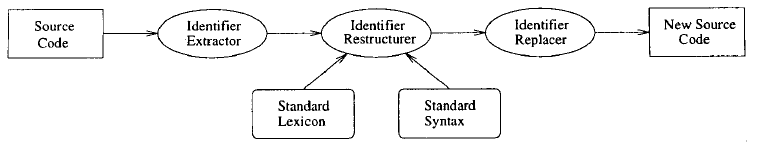
\includegraphics[scale= 0.80]{./ire_1.png}
}
\caption{Etapas de Restructuring tool}
\label{ire1}
\end{figure}

La herramienta Restructuring Tool \cite{BCPT00} se encarga de recibir como entrada un código fuente escrito en lenguaje C. Luego a través de un proceso de transformación cada id del código se expande a palabras completas. La salida es el mismo código pero con los ids expandidos.
Cabe destacar que esta herramienta es semi-automática, en algunas situaciones necesita intervenir el usuario.

Los ids se cambian por nombres más explicativos, los cuales incluyen un verbo que indica la función del id en el código. Más precisamente después de renombrar los ids se visualiza claramente el rol que cumple el id en el programa.

El código fuente se convierte de esta manera en un código más entendible y mejora la comprensión. El proceso consta de tres etapas (Figura \ref{ire1}): 

\begin{enumerate}
\itemsep0em%reduce espacio
\item \textbf{Identifier Extractor:} Recupera una lista con los nombres de los ids presentes en el código. Este módulo se programó con un parser modificado de C que reconoce los ids y los extrae.
\item \textbf{Identifier Restructurer:} Genera una asociación entre el nombre actual del id y un nuevo nombre estándar expandido. El primer paso consiste en segmentar el id en las palabras que lo constituyen. Después, cada palabra se expande usando un diccionario de palabras estándar (estándar léxico). Finalmente, la secuencia de palabras expandidas deben coincidir con reglas predefinidas por una gramática para determinar que acción cumple el id en el código \mbox{(estándar sintáctico).}
\item \textbf{Identifier Replacer:} Transforma el código original en el nuevo código usando las asociaciones que se construyeron en la etapa anterior. Se emplea un scanner léxico para evitar reemplazar posibles nombres de ids contenidos en literales strings y en comentarios.
\end{enumerate}

Los pasos 1 y 3 están totalmente automatizados. Sin embargo, para lograr que la expansión de nombres sea efectiva, se necesita que en algunos casos del paso 2 intervenga el usuario.

\begin{figure}[h] %[h] para here [b] para bottom [t] para top
\centering
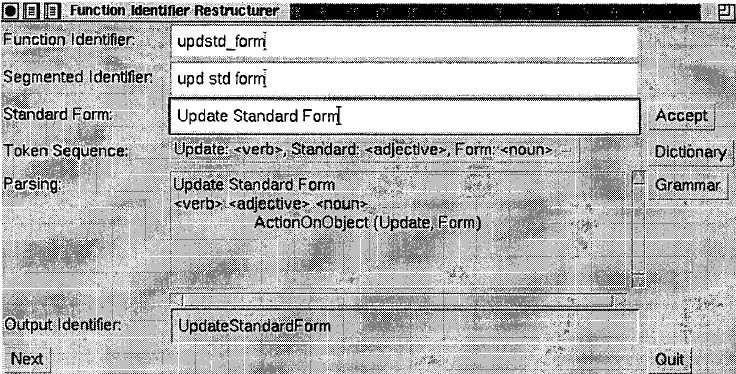
\includegraphics[scale= 0.60]{./ire_2.png}
\caption{Etapas de Identifier Restructurer.}
\label{ire2}
\end{figure}

A continuación, se detalla el paso 2 que es el más importante de esta herramienta, en la Figura \ref{ire2} se desglosa las diferentes etapas.

\begin{description}
\itemsep0em%reduce espacio
\item[Segmentation:] El id se separa en las palabras que lo componen. De manera automática se utilizan estrategias simples de separación (basada en guión bajo o camel-case: hardword - ejemplo: \textsf{get\_txt} $\rightarrow$ \textsf{get txt}). En caso presencia de softwords, la división se debe hacer en forma manual. Por ejemplo: \textsf{get\_txtinput} $\rightarrow$ \textsf{get txt input} la separación entre \textsf{txt} e \textsf{input} la realiza el usuario. De manera conceptual (no implementado), los autores proponen automatizar más esta fase. La propuesta consiste de un algoritmo hecho en LISP, este toma un string \textit{s} como entrada. Se utiliza una estrategia greedy verificando a partir de la primer letra de \textit{s} un sub-string que pertenezca a un diccionario predefinido. Luego el sub-string se descarta y continúa el análisis con el resto hasta que no haya más sub-strings que separar \cite{BCPT99}.

\begin{figure}[h] %[h] para here [b] para bottom [t] para top
\centerline{%queda centrada mejor la imagen
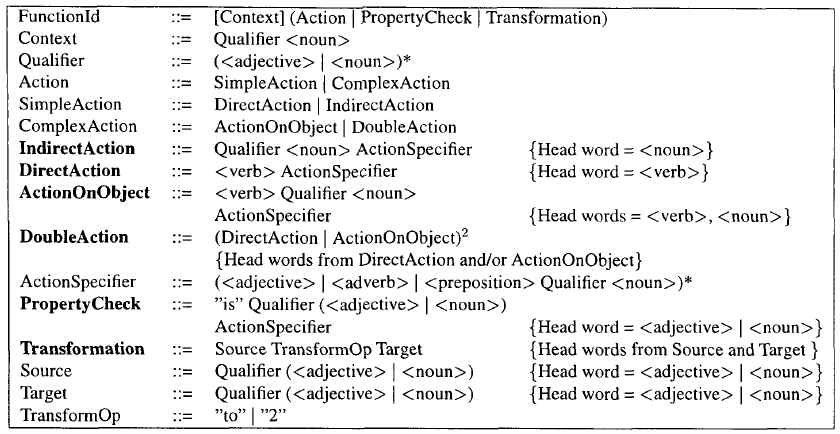
\includegraphics[scale= 0.60]{./ire_3.png}
}
\caption{Gramática que determina la función de los ids.}
\label{ire3}
\end{figure}

\item[Standard Lexicon:] Una vez lograda la separación de las palabras estas son mapeadas a una forma estándar (expandidas) con la ayuda de un diccionario léxico \cite{BCPT99} (Ejemplo: \textsf{upd} $\rightarrow$ \textsf{Update}). Una idea de mejora propuesta es incorporar al diccionario términos extraídos del código fuente. También aquí, el usuario puede intervenir para realizar la expansión manualmente. Los autores \cite{BCPT00} de la herramienta construyeron los diccionarios de manera genérica tomando como muestra 10 programas. Sin embargo, se aconseja que con el tiempo los diccionarios deben crecer con la inclusión de nuevos términos.

\item[Tokenization:] Una vez obtenidas las palabras a una forma estándar (expandida) en el paso anterior, se procede a asignar cada palabra a un \textit{tipo léxico} (verbo, sustantivo, adjetivo). Por ejemplo, la palabra \textsf{Update} se transforma en $<$Update,verb$>$, \textsf{Standard} a $<$Standard,adjective$>$. Esta tuplas se denominan tokens y se utiliza un `diccionario de tipos' para generarlos de manera automática, este diccionario al igual que los otros se arma previamente a gusto del programador \cite{BCPT99}. Sin embargo, existen casos que se necesita la intervención humana para determinar el tipo correcto. Por ejemplo, \textsf{free} en inglés es un verbo, un adjetivo y a la vez un adverbio.% En este caso la herramienta va a elegir lo que el diccionario le indique (si free esta presente).

\item[Parsing:] Finalmente, la secuencia de tokens obtenidos en la etapa anterior se parsea usando una gramática predefinida. Este parseo permite determinar cuál es el rol/acción del id en el código fuente y de esta manera, se determina la “acción semántica” del id. 
En la figura 3.8 se muestra un ejemplo de gramática construida por los autores. Cabe aclarar que cada usuario puede elaborar su propia gramática. 
Es una gramática regular donde los símbolos terminales están indicados con $<>$. Las producciones con negrita, determinan en función del tipo léxico asignado a cada palabra la acción semántica del id.
Por ejemplo, el verbo expresa la acción y el sustantivo representa al objeto de la acción, con \textbf{ActionOnObject} $\Rightarrow$ $<$verb$>$,$<$noun$>$ $\equiv$ $<$go,home$>$. Otro ejemplo es, \textbf{IndirectAction} $\Rightarrow$ $<$adjetive$>$,$<$noun$>$ $\equiv$ $<$order,textfield$>$ donde el adjetivo representa una cualidad del sustantivo.

En caso de que el parseo falle el proceso se reinicia desde el comienzo partiendo nuevamente de la etapa de segmentación \cite{BCPT00} (figura \ref{ire2}).
\end{description}

\begin{figure}[ht] %[h] para here [b] para bottom [t] para top
\centering
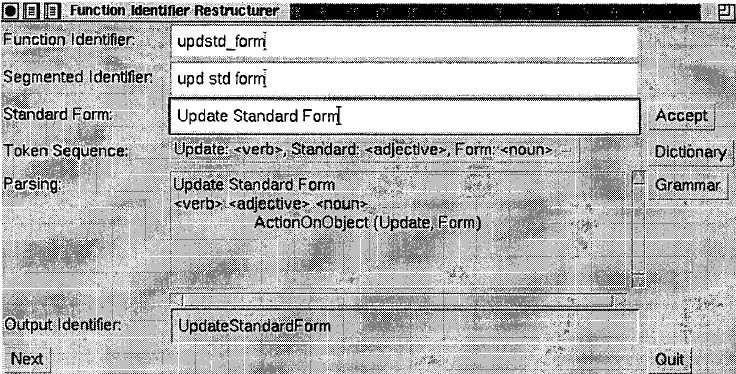
\includegraphics[scale= 0.67]{./ire_4.png}
\caption{Visualización de Restructuring Tool.}
\label{ire4}
\end{figure}

\pagebreak
\noindent \textbf{Interfaz para el Usuario\\}

La interfaz para el usuario de \textbf{Identifier Restructurer} se visualiza en la figura \ref{ire4}, el id de entrada se muestra en el primer cuadro de texto \textsf{updstd\_form}. Se usan heurísticas sencillas (guión bajo, camel-case) para separar las palabras del id, en este caso \textsf{updstd} y \textsf{form}. Como esta segmentación está incompleta, el usuario puede separar manualmente en el segundo cuadro de texto la palabra \textsf{upd} y \textsf{std} (ver figura \ref{ire4}). En el tercer cuadro de texto se propone la forma estándar de cada palabra. Cuando una palabra no se puede expandir la herramienta muestra un signo de pregunta en su lugar (?). En este caso \textsf{upd} $\rightarrow$ \textsf{Update}, \textsf{std} $\rightarrow$ (?), \textsf{form} $\rightarrow$ \textsf{Form}, como \textsf{std} no está presente en el diccionario se necesita la intervención del desarrollador para que se complete correctamente a \textsf{Standard}. Luego las palabras expandidas son asociadas a la función gramatical. En esta etapa puede existir para una secuencia de palabras más de una función gramatical (la gramática es ambigua y puede generar más de una secuencia de tokens). En caso de suceder esto el usuario puede elegir cual es la secuencia más adecuada. En el ejemplo de la figura \ref{ire4} solo existe una única función gramatical y es reflejada en el cuarto cuadro de texto. 

Luego, en el cuadro de Parsing se puede apreciar la acción que aplica el id, en este caso \textbf{ActionOnObject(Update,Form)} `actualizar formulario'. Finalmente el resultado se detalla en el último cuadro de texto de más abajo.

Cuando se arma la asociación de los nombres ids con los nuevos nombres generados la misma debería cumplir con la propiedad de inyectividad, de esta forma se evita que haya conflictos de nombres entre los distintos ids del programa. La herramienta ayuda al programador a conseguir este objetivo resaltando los posibles conflictos en los nombres.

Para concluir, la etapa \textbf{Identifier Replacer} toma todas las ocurrencias del id \textsf{updstd\_form} y se reemplaza por \textsf{UpdateStandarForm}, como se mencionó con anterioridad.

\section{Conclusiones}

Las observaciones que se destacan en el estado del arte de las técnicas de análisis de ids apuntan por un lado al nombramiento correcto de los ids. Al comienzo de este capítulo se detalló una herramienta que ayuda a lograr esta meta. Sin embargo, no trascendió ya que es costosa de utilizar sobre grandes proyectos de software y solo es efectiva cuando se emplea desde el arranque del desarrollo de un sistema.

El correcto nombramiento en los ids es crucial para la comprensión de los sistemas, un código con ids más descriptivos y claros se entiende mucho mejor. Además en este contexto, las herramientas/técnicas de análisis de ids mejoran sus resultados. De esta manera, es más sencillo extraer conceptos del dominio del problema desde los ids.

Las herramientas/técnicas de análisis de ids han ido evolucionando con el pasar del tiempo. Al principio algunas etapas necesitaban la intervención del usuario para realizar las tareas, se puede decir que usaban procesos semi-automatizados. A medida que se construyeron nuevas técnicas, se buscó más la automatización haciendo que el programador se involucre menos.

Como se mencionó en este capítulo, las primeras técnicas utilizaban netamente diccionarios de palabras en lenguaje natural, lo cual requiere mucho espacio de almacenamiento. Más tarde, se intentó disminuir el uso de estos diccionarios mirando más los recursos internos de información dentro los sistemas, como es el caso de los comentarios, literales strings y la documentación.

Sin embargo, suele ocurrir que estos recursos internos son escasos. Es por esto, que los autores de las recientes técnicas decidieron recurrir a procesos que examinan programas de gran envergadura. Estos procesos recolectan palabras útiles que son almacenadas en forma de diccionarios. Estos diccionarios no solo ayudan a traducir el significado de los ids, también tiene bajas exigencias de almacenamiento y están constituidos con palabras más adecuadas al ámbito de las ciencias de la computación.


%Con este estudio se puede observar que los ids son una fuente importante de información, por eso elaborar técnicas que analicen ids es un aporte destacado para la CP.

%\section{Técnicas de División de Identificadores}
%\section{Técnicas de Expansión de Identificadores}

%En el área de Ingeniería del Software, existen herramientas automatizadas que permiten hacer análisis de los identificadores utilizados en los códigos de programación. Estas herramientas extraen parcialmente conceptos representados en los identificadores del código fuente para intentar interpretar lo que el programador quiso desarrollar.

%Estas técnicas exhiben información estática oculta detrás de los ids, esta información es importante porque da indicios de lo que un sistema realiza en su ejecución por ende es un aporte en el ámbito de Comprensión de Programas. --colocar abajo

%========================================================================
\chapter{Identifier Analyzer (IDA)}

\section{Arquitectura}

La herramienta IDA esta implementada con lenguaje JAVA y fue desarrollada usando el entorno de desarrollo NetBeans. IDA posee dos fuentes de entrada; una fuente corresponden a archivos  escritos en JAVA, la otra fuente corresponden a archivos escritos en XML.  

\pagebreak
\begin{figure}[ht] %[h] para here [b] para bottom [t] para top
\centering
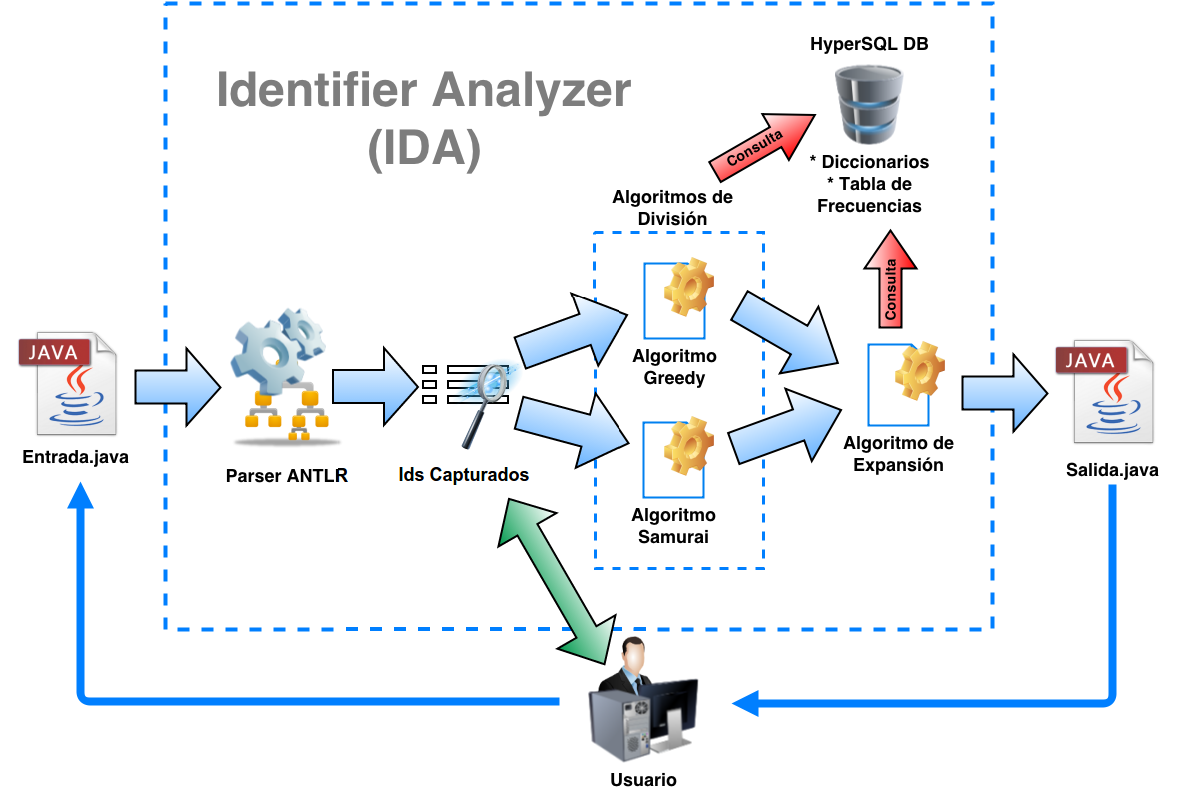
\includegraphics[scale= 0.35]{./ida_arq.png}
\caption{Arquitectura de IDA.}
\label{ire4}
\end{figure}

\bibliographystyle{plain}%{alpha}
\bibliography{biblo.bib}

\end{document}
